
\chapter{Desenvolvimento}

Este capítulo apresenta a visão geral do jogo proposto, seus requisitos e principais elementos, como personagens e ambientes. Também são detalhados os objetivos e mecânicas do jogo e suas cenas. Finalmente, é apresentada a operacionalização do jogo.

\section{Visão Geral}

O jogo é chamado ``Mistério Financeiro: A Jornada de Chico''. No início o protagonista Chico se depara com o mistério das despesas crescentes e do desaparecimento de moedas na papelaria de sua família. Motivado por um senso de responsabilidade, ele decide investigar o caso. A investigação começa pelo porão da loja, um local pouco visitado pela sua família.

A narrativa avança através de uma série de desafios e escolhas que Chico deve enfrentar. Essas decisões vão desde escolhas cotidianas, como a compra de um relógio, até interações complexas com personagens, como seu amigo Vicente. Cada escolha tem um impacto na história e nas lições de economia e gestão financeira apresentadas.

À medida que Chico investiga, ele descobre várias causas para os problemas financeiros da papelaria, desde descuidos simples até ações mal-intencionadas de terceiros. O jogo ressalta a importância da atenção aos detalhes e do controle de gastos para a saúde financeira de um negócio.

O jogo é estruturado de forma interativa, oferecendo múltiplos finais baseados nas decisões do jogador ao longo de sua experiência. Isso enfatiza a relevância de escolhas responsáveis e informadas, tanto no jogo quanto na vida real. Neste sentido, o jogo incorpora um forte elemento educacional, enfatizando conceitos de gestão financeira. Ele ensina sobre a importância do planejamento financeiro, economia e investimentos, incentivando os jogadores a refletirem sobre suas próprias decisões financeiras.

\section{Requisitos de Software}

\subsection*{Requisitos Funcionais}
\begin{itemize}
	\item RF1. O jogo deve oferecer uma interface gráfica interativa, simbolizando os diferentes ambientes da história de Chico.
	\item RF2. Incluir um sistema de diálogo interativo com personagens, como Seu Mário, Vicente, Luiza, entre outros.
	\item RF3. Permitir que o jogador faça escolhas que influenciam o desenvolvimento da história e interações com personagens.
	\item RF4. Permitir a compra e uso de itens para progredir na narrativa, principalmente se tratando da lanterna que será usada para verificar o porão.
	\item RF5. Apresentar múltiplos finais com base nas decisões tomadas pelo jogador, influenciadas pelas interações com personagens.
	\item RF6. Incorporar elementos de educação financeira dentro da narrativa e desafios, utilizando situações da história de Chico como exemplos.
\end{itemize}

\subsection*{Requisitos Não Funcionais}
\begin{itemize}
	\item RNF1. O jogo deve ter uma interface gráfica atrativa e intuitiva, adequada para a faixa etária do 5º ano do Ensino Fundamental.
	\item RNF2. O jogo deve ser otimizado para um desempenho fluido, sem atrasos ou erros técnicos.
	\item RNF3. O jogo deve ser compatível com a plataforma Windows, MacOS e Web.
	\item RNF4. O jogo deve ter uma trilha sonora e efeitos sonoros imersivos, complementando a experiência visual.
\end{itemize}

\subsection*{Regras de Negócio}
\begin{itemize}
	\item RN1. A história deve se adaptar e mudar com base nas escolhas feitas pelo jogador (RF3, RF5).
	\item RN2. Os desafios e enigmas devem ser integrados na história e contribuir para o aprendizado sobre finanças (RF4, RF6).
	\item RN3. Os diálogos e interações com personagens devem oferecer pistas e informações relevantes para a progressão da história (RF2).
	\item RN4. O jogo deve promover a conscientização sobre gestão financeira e economia de forma lúdica e educativa (RF6).
	\item RN5. Os elementos e enredo do jogo devem seguir a história 1 do livro 5 da ENEF, garantindo alinhamento com os princípios educativos estabelecidos.
\end{itemize}

\section{Detalhamento do Jogo}

\subsection{Personagens e Ambientes}
Esta seção detalha os personagens não jogáveis (NPCs, do inglês \textit{non-player character}) e os ambientes (também chamados de \textit{mapas}) que serão fundamentais para a narrativa e jogabilidade do jogo. Cada NPC e mapa pode ser acompanhado de uma imagem e uma descrição detalhada para melhor imersão e compreensão do jogador.

O jogo apresenta os NPCs apresentados na Figura~\ref{fig:npcs}. Abaixo, é fornecida uma descrição para cada um deles.

\medskip\noindent \textbf{Seu Mário.}\quad Pai de Chico, dedicado dono da papelaria da família. Enfrenta desafios financeiros e tenta manter o negócio próspero.

\medskip\noindent \textbf{Pai do Vicente.}\quad Aparece na história para repreender seu filho por envolvimento em furtos, refletindo preocupação paterna diante da situação indesejada.

\medskip\noindent \textbf{Atendente da Loja de Itens.}\quad Caracterizado como um comerciante prestativo, interage com Chico durante a compra do seu relógio.

\medskip\noindent \textbf{Vicente.}\quad Colega de escola de Chico, conhecido por seu comportamento provocativo e envolvimento em pequenos furtos.

\medskip\noindent \textbf{Luiza.}\quad Melhor amiga de Chico, sempre oferecendo apoio e aconselhamento nas aventuras e desafios enfrentados por ele.

\medskip\noindent \textbf{Maria José.}\quad Mãe de Chico, auxilia na papelaria e compartilha das preocupações financeiras da família.

\medskip\noindent \textbf{Josimar.}\quad Funcionário da papelaria, inicialmente suspeito de furto, revelando-se inocente e um aliado importante.

\medskip\noindent \textbf{Ratazana.}\quad Uma ameaça inesperada no porão da papelaria, adicionando suspense e desafios físicos à narrativa.

\medskip\noindent \textbf{Atendente do Hospital.}\quad Representa um ponto de contato no cenário hospitalar, caso Chico necessite de cuidados médicos devido ao ataque da ratazana.

\medskip\noindent \textbf{Médico.}\quad Figura de cuidado e autoridade, que atende Chico no hospital após eventuais incidentes.

\medskip\noindent \textbf{Atendente da Loja de Ferragens.}\quad Ajuda Chico na aquisição da lanterna, útil durante suas investigações.

\medskip\noindent \textbf{Cida.}\quad Irmã mais nova de Chico, envolvida nos dilemas familiares e curiosa sobre os mistérios da papelaria.

\medskip\noindent \textbf{Personagens não nomeados (4).}\quad Personagens secundários, aparecem apenas para compor algumas cenas, como o encontro com os amigos da escola na lanchonete.


\begin{figure}[ht]
	\centering
	\caption{Imagens de cada NPC.}
	
\includegraphics[scale=1.0]{Textuais/Pictures/NPC-Todos.png}
	\fonte{Criado pelo autor.}\label{fig:npcs}
\end{figure}

\newpage

\bigskip\medskip
O jogo ainda apresenta nove ambientes, os quais estão apresentados nas Figuras~\ref{fig:mundo-chico}~--~\ref{fig:hospital}. Os detalhes de cada ambiente são fornecidos abaixo.

\medskip\noindent \textbf{Mundo do Chico.}\quad O cenário geral da aventura, que inclui a vizinhança, ruas e locais frequentados por Chico e seus amigos (Figura~\ref{fig:mundo-chico}).

\medskip\noindent \textbf{Casa do Chico.}\quad Espaço de união e diálogo da família, proporcionando um contraste com as áreas de mistério e aventura (Figura~\ref{fig:casa-chico}).

\medskip\noindent \textbf{Loja de Itens.}\quad Estabelecimento onde Chico adquire itens como o relógio (Figura~\ref{fig:loja-itens}).

\medskip\noindent \textbf{Lanchonete.}\quad Espaço social para Chico e seus amigos, propício para conversas e desenvolvimento de subtramas (Figura~\ref{fig:lanchonete}).

\medskip\noindent \textbf{Loja de Ferragens.}\quad Fornecedora da lanterna para as investigações de Chico (Figura~\ref{fig:loja-ferragens}).

\medskip\noindent \textbf{Papelaria da Família.}\quad Coração da trama, onde muitos dos mistérios e desafios se concentram (Figura~\ref{fig:papelaria-familia}).

\medskip\noindent \textbf{Cozinha da Papelaria.}\quad Local onde Chico encontra o Josimar e faz descobertas, como o problema com a geladeira (Figura~\ref{fig:cozinha-papelaria}).

\medskip\noindent \textbf{Porão da Papelaria.}\quad Ambiente sombrio e cheio de mistérios, onde Chico enfrenta a Ratazana (Figura~\ref{fig:porao-papelaria}).

\medskip\noindent \textbf{Hospital.}\quad Local de cuidado e recuperação, podendo ser cenário de eventos dramáticos, como o ataque da ratazana (Figura~\ref{fig:hospital}).


\begin{figure}[!htbp]
	\centering
	\caption{Mapa Mundo Chico.}
	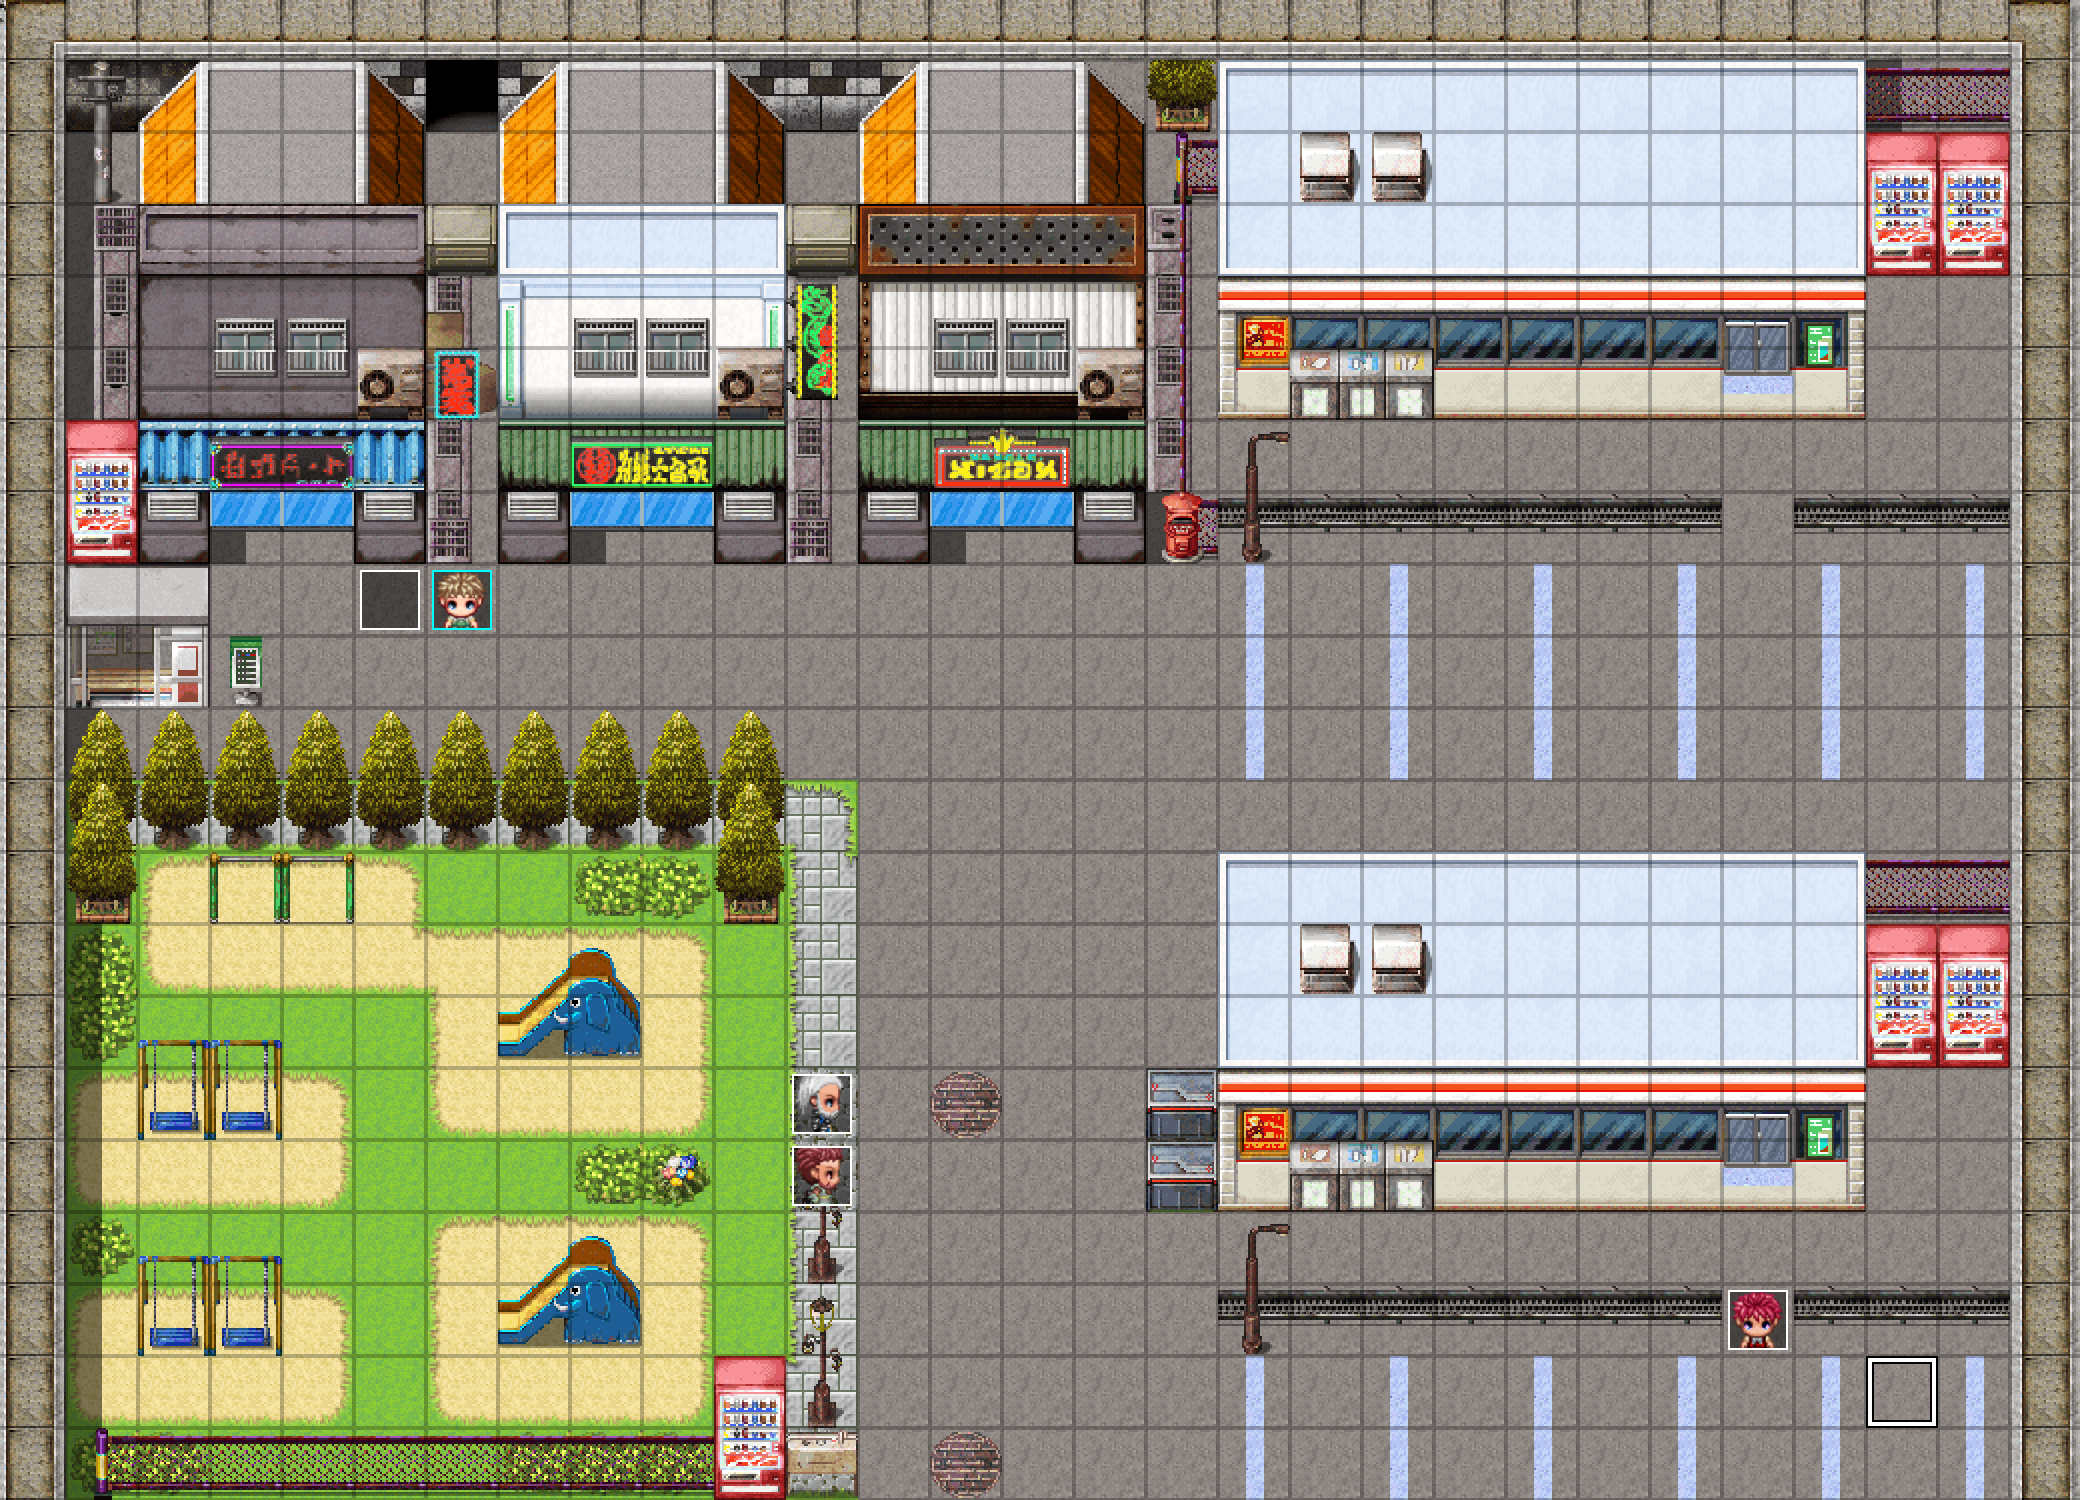
\includegraphics[scale=0.4]{Textuais/Pictures/Mundo_chico.png}
	\fonte{Criado pelo autor com base nos modelos fornecidos pelo RPG Maker MZ.}\label{fig:mundo-chico}
\end{figure}

\begin{figure}[!htbp]
	\centering
	\caption{Mapa da casa do Chico.}
	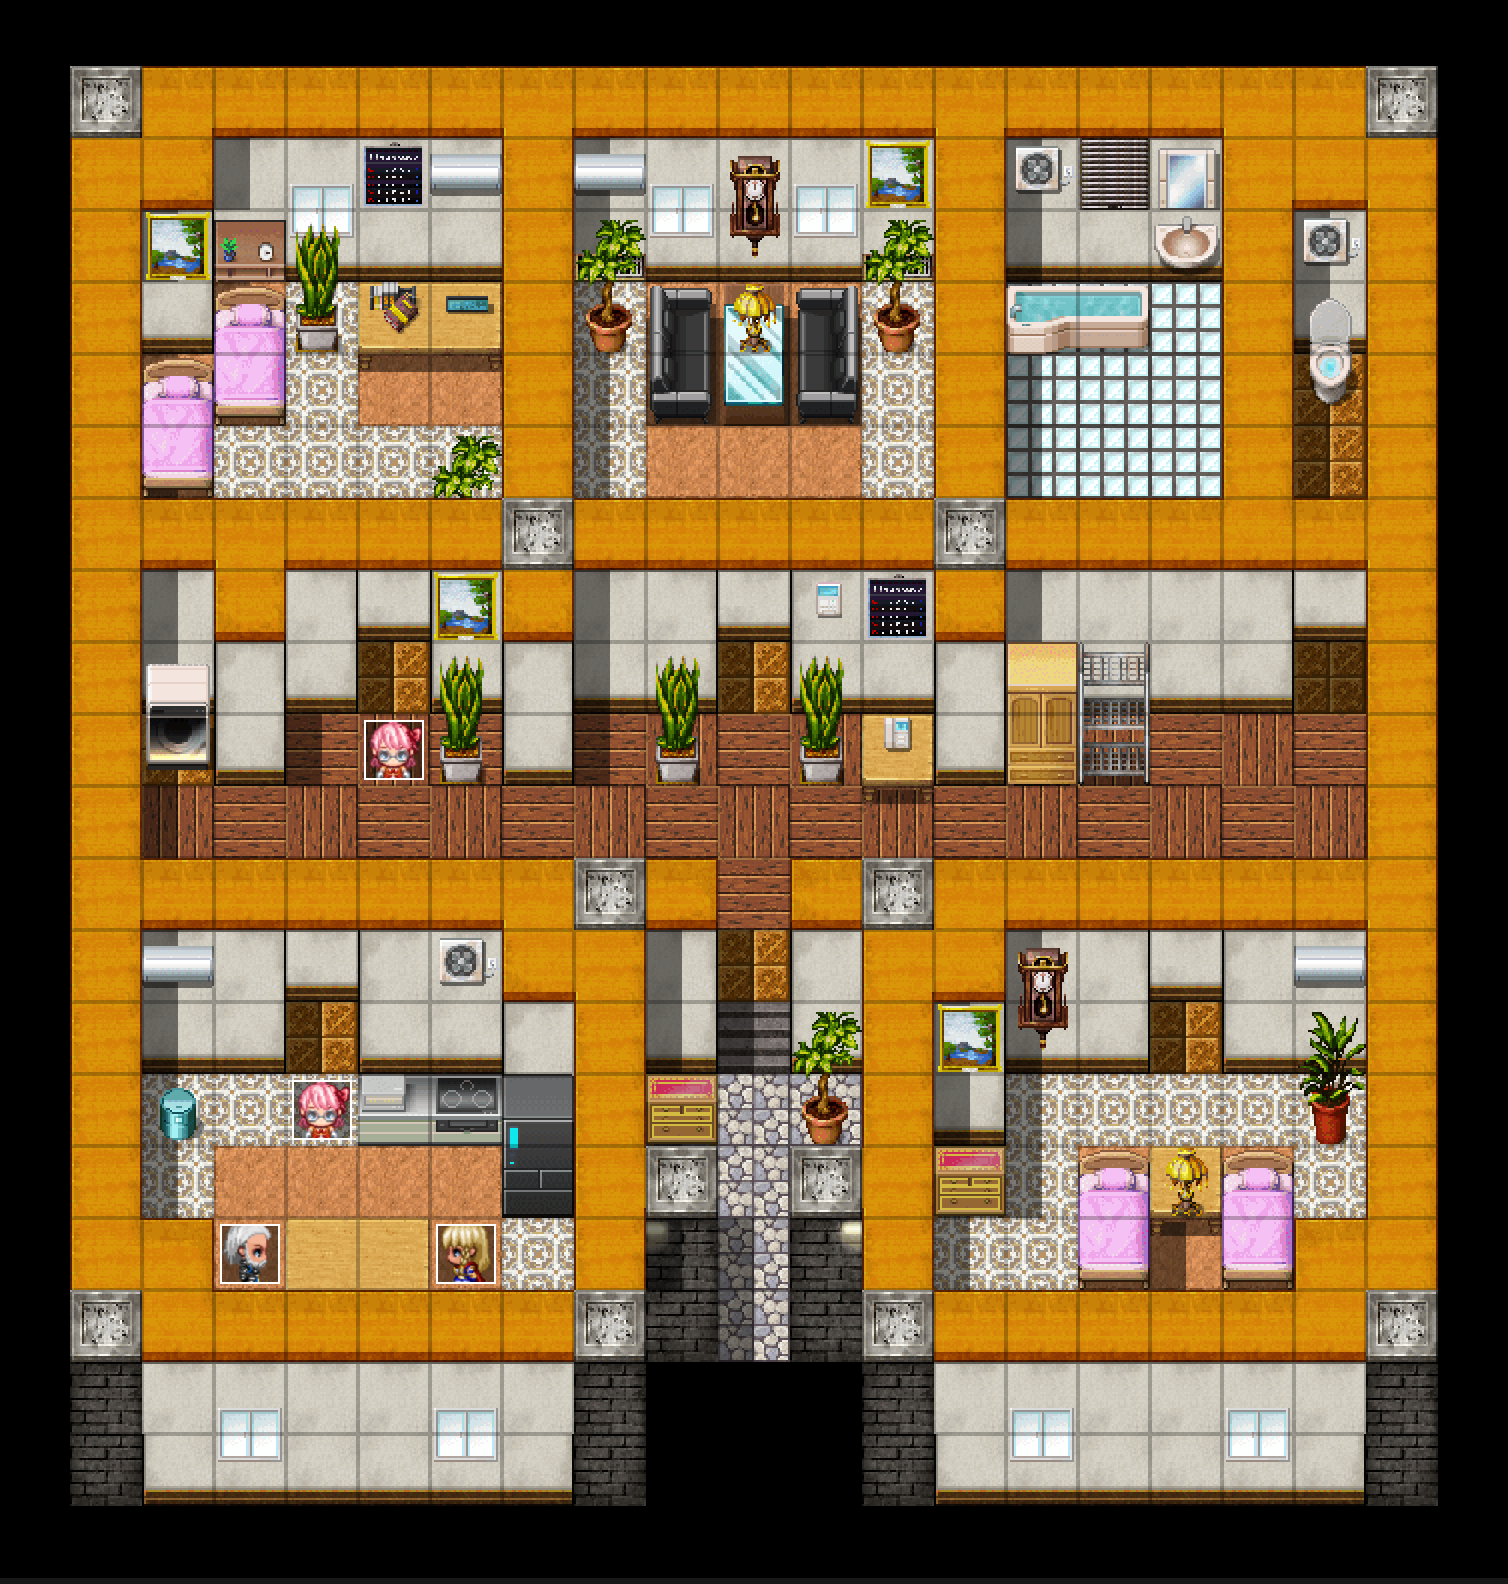
\includegraphics[scale=0.35]{Textuais/Pictures/Casa_chico.png}
	\fonte{Criado pelo autor com base nos modelos fornecidos pelo RPG Maker MZ.}\label{fig:casa-chico}
\end{figure}

\begin{figure}[!htbp]
	\centering
	\caption{Mapa Loja de Itens.}
	\includegraphics[scale=0.5]{Textuais/Pictures/Loja_itens.png}
	\fonte{Criado pelo autor com base nos modelos fornecidos pelo RPG Maker MZ.}\label{fig:loja-itens}
\end{figure}

\begin{figure}[!htbp]
	\centering
	\caption{Mapa Lanchonete.}
	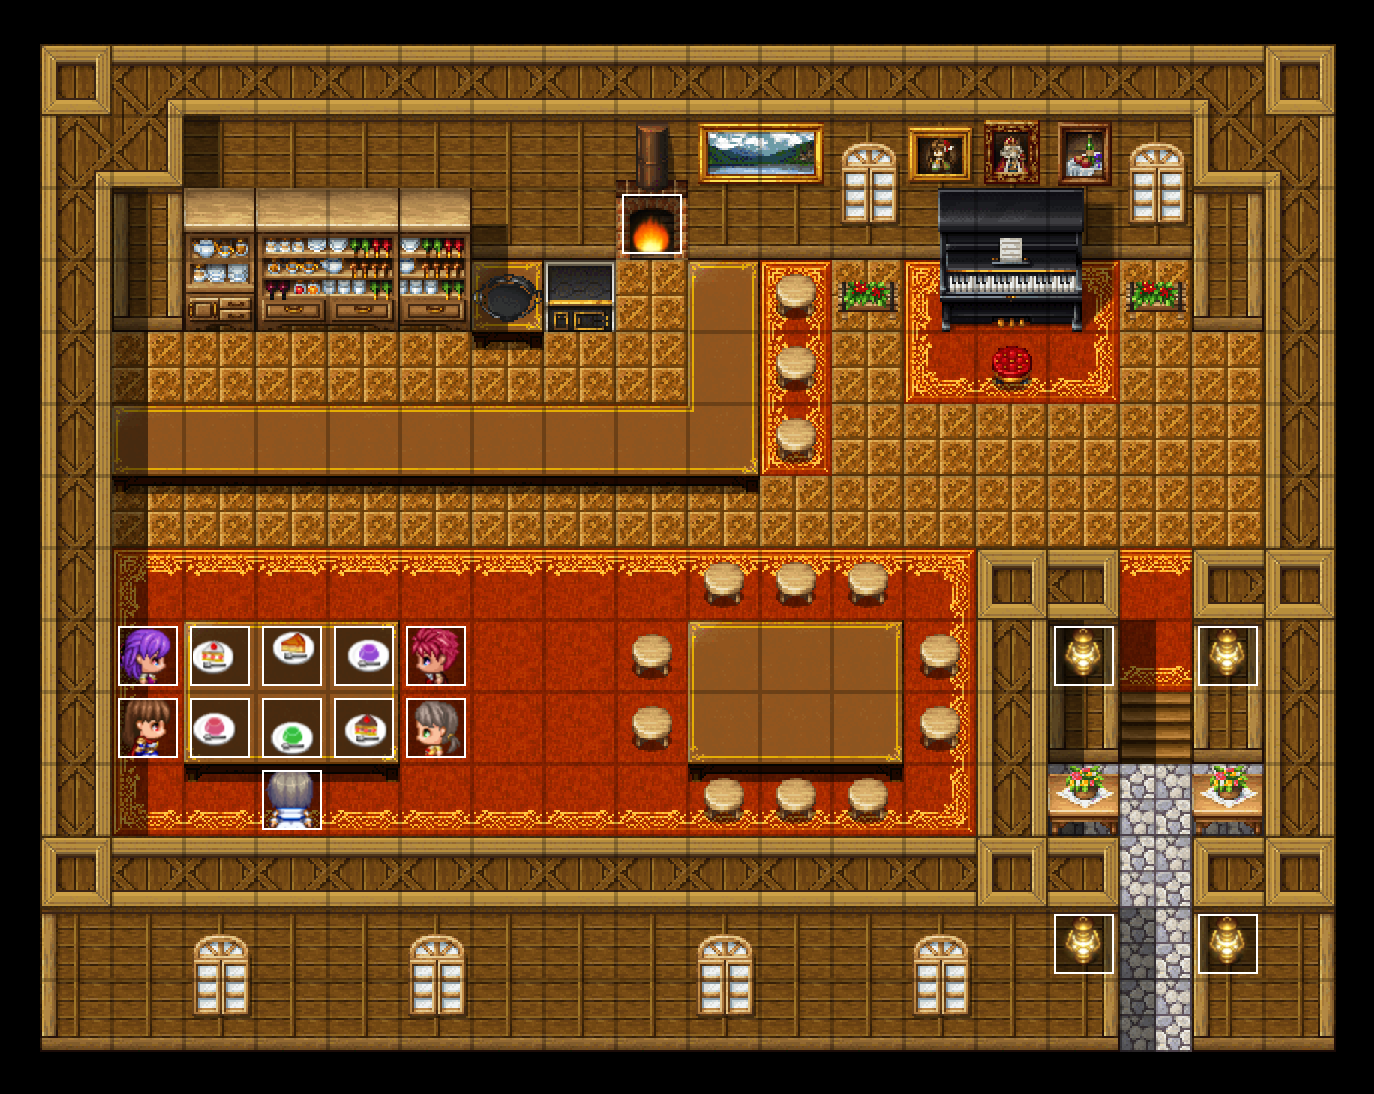
\includegraphics[scale=0.5]{Textuais/Pictures/Lanchonete.png}
	\fonte{Criado pelo autor com base nos modelos fornecidos pelo RPG Maker MZ.}\label{fig:lanchonete}
\end{figure}

\begin{figure}[!htbp]
	\centering
	\caption{Mapa da loja de ferragens.}
	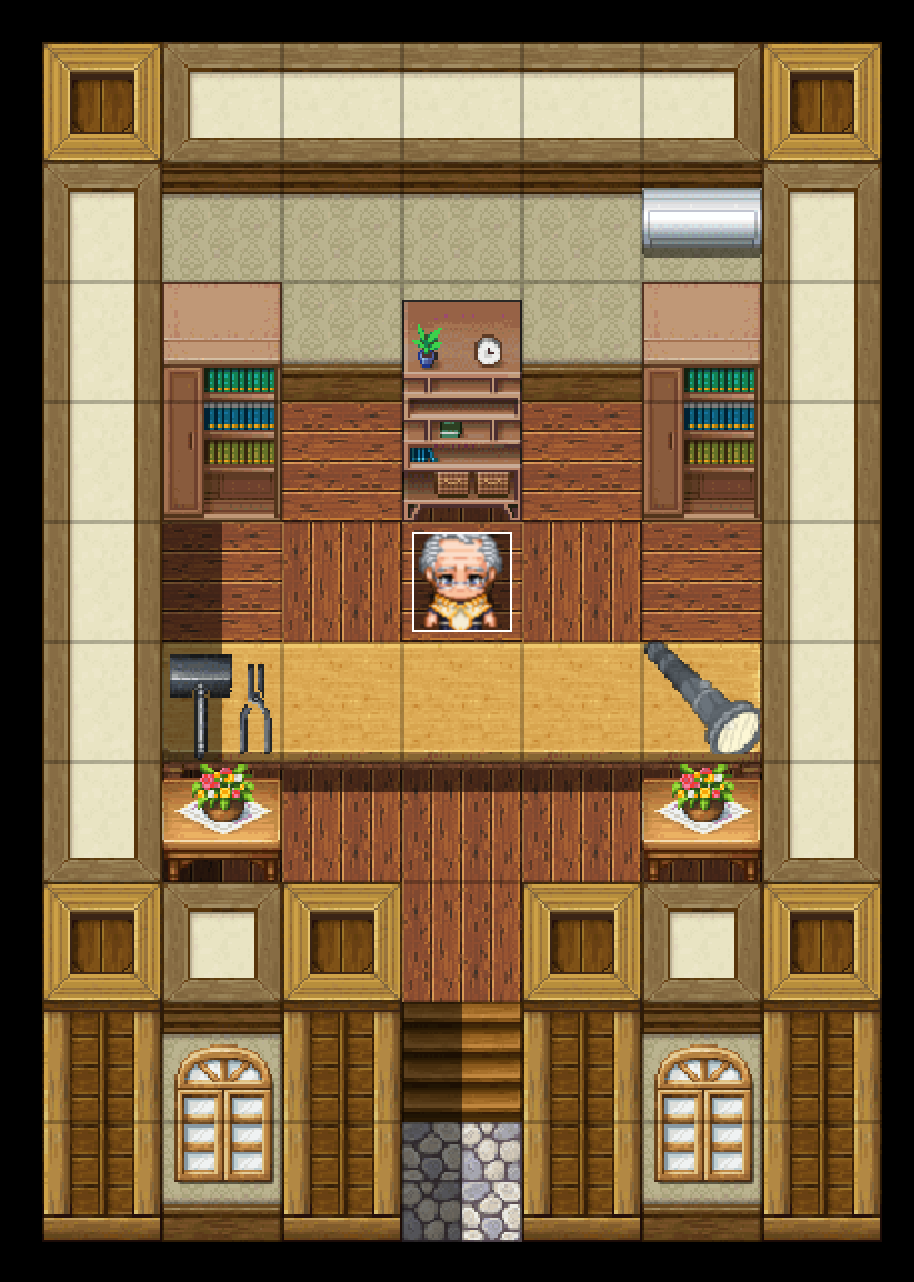
\includegraphics[scale=0.45]{Textuais/Pictures/Loja_Ferragens.png}
	\fonte{Criado pelo autor com base nos modelos fornecidos pelo RPG Maker MZ.}\label{fig:loja-ferragens}
\end{figure}

\begin{figure}[!htbp]
	\centering
	\caption{Mapa Papelaria.}
	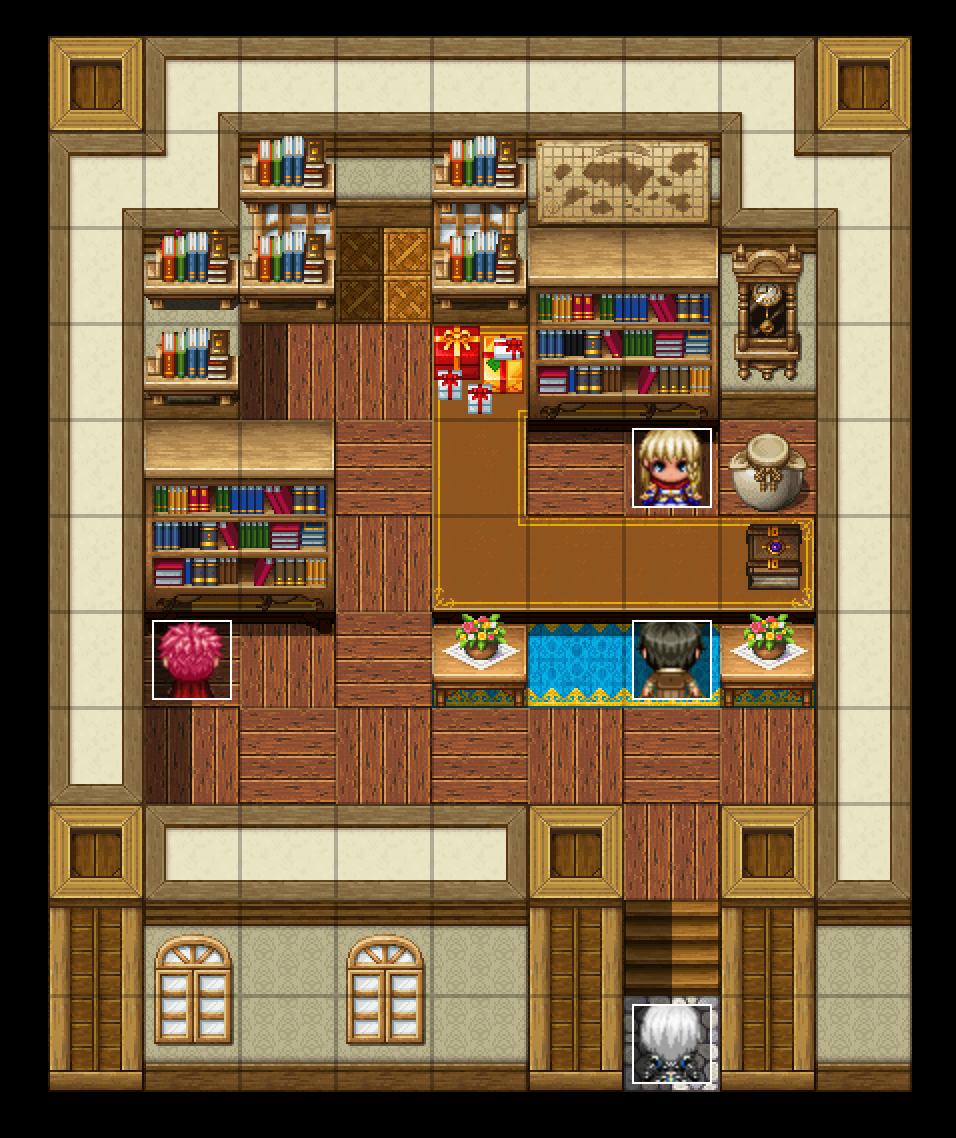
\includegraphics[scale=0.45]{Textuais/Pictures/Papelaria_Familia.png}
	\fonte{Criado pelo autor com base nos modelos fornecidos pelo RPG Maker MZ.}\label{fig:papelaria-familia}
\end{figure}

\begin{figure}[!htbp]
	\centering
	\caption{Mapa da cozinha da papelaria.}
	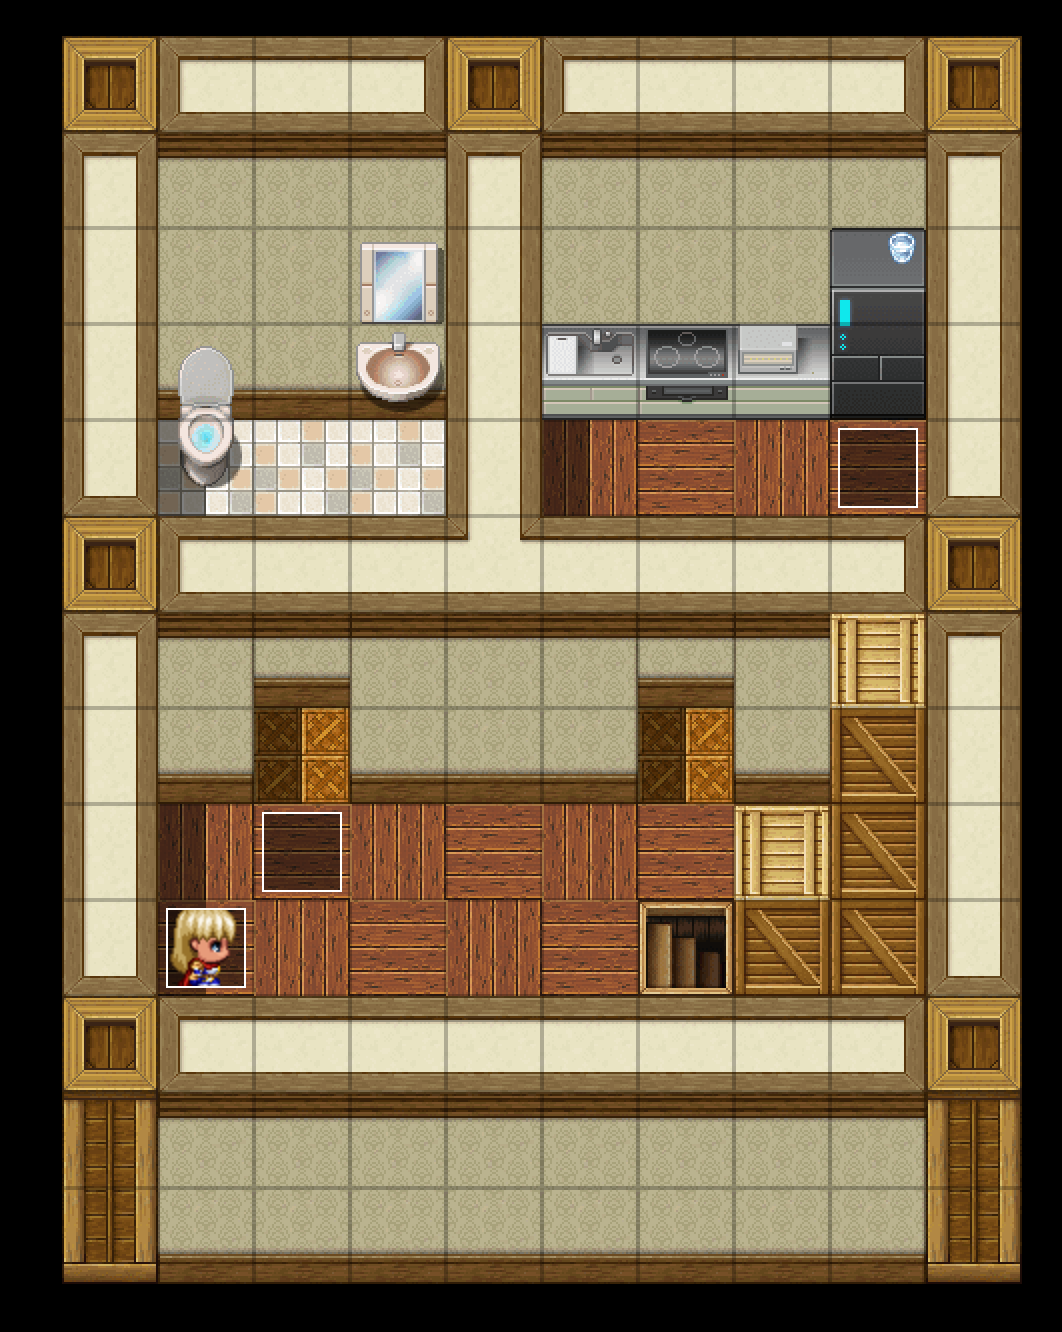
\includegraphics[scale=0.5]{Textuais/Pictures/Cozinha_papelaria.png}
	\fonte{Criado pelo autor com base nos modelos fornecidos pelo RPG Maker MZ.}\label{fig:cozinha-papelaria}
\end{figure}

\begin{figure}[!htbp]
	\centering
	\caption{Mapa do porão da papelaria.}
	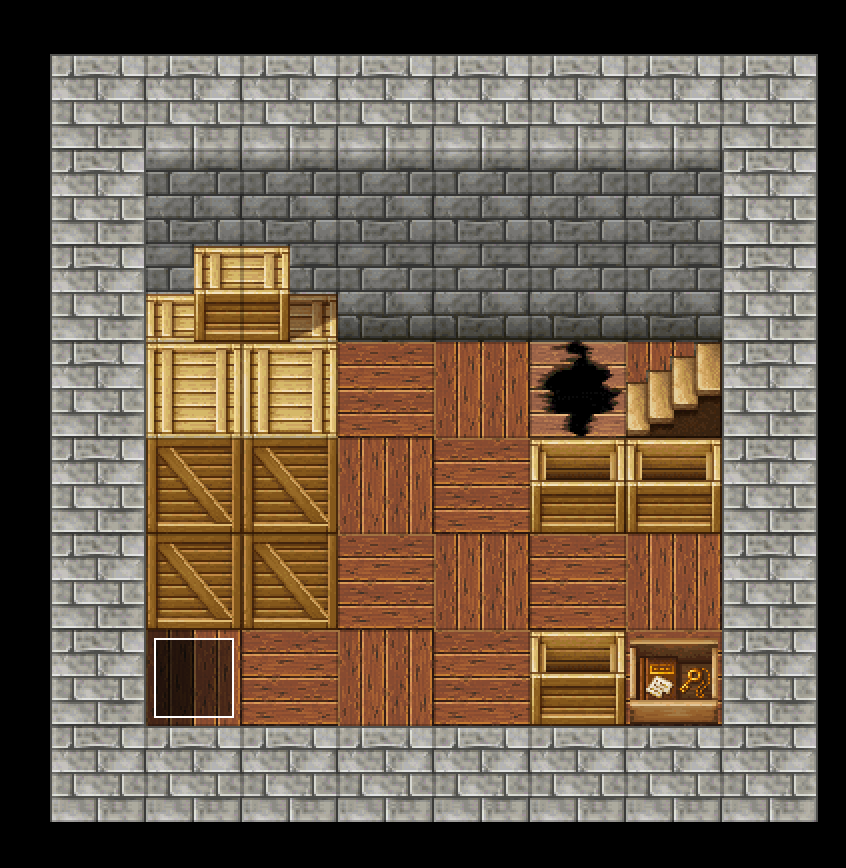
\includegraphics[scale=0.5]{Textuais/Pictures/Porao_papelaria.png}
	\fonte{Criado pelo autor com base nos modelos fornecidos pelo RPG Maker MZ.}\label{fig:porao-papelaria}
\end{figure}

\begin{figure}[!htbp]
	\centering
	\caption{Mapa do hospital.}
	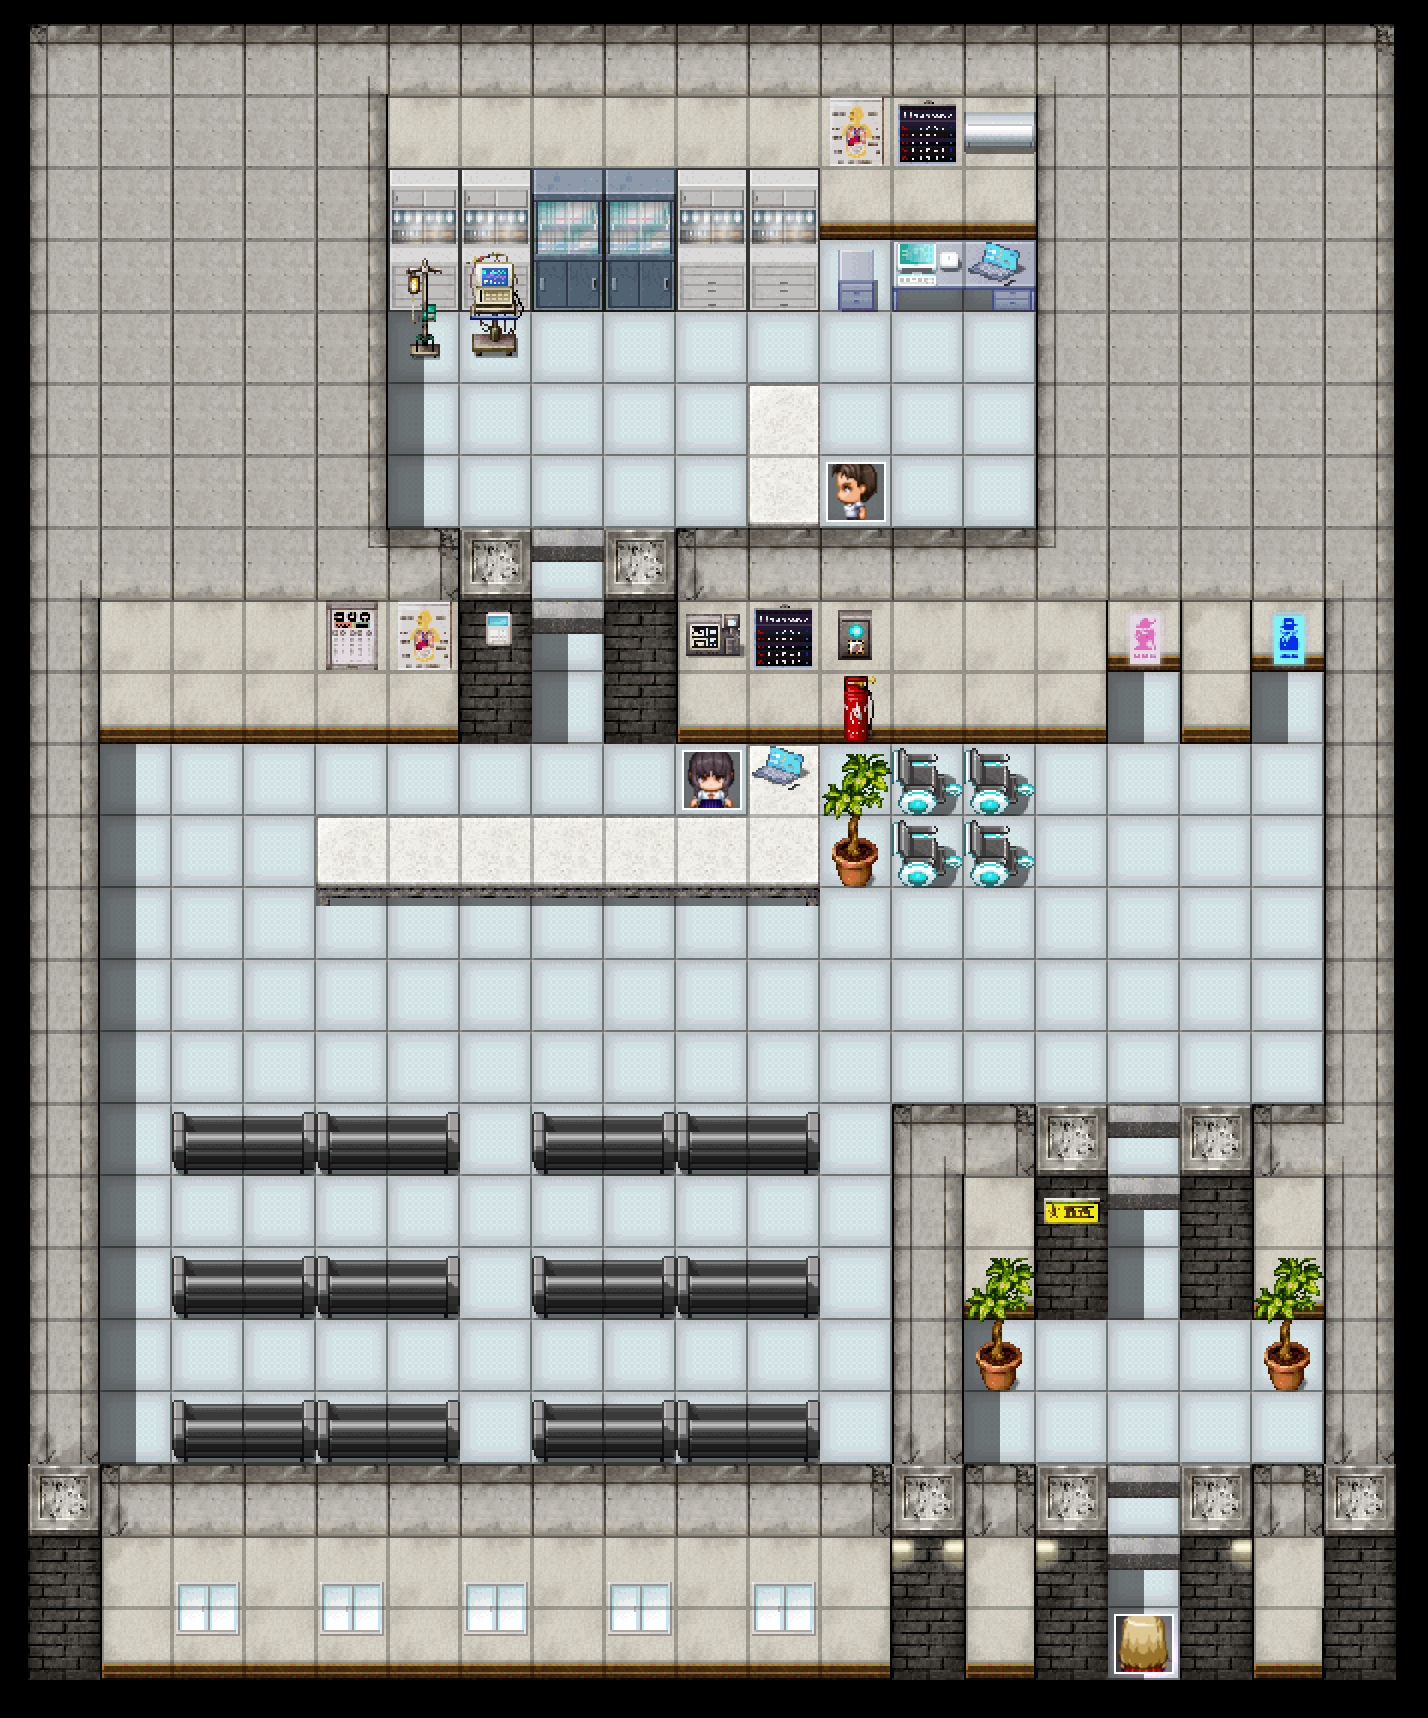
\includegraphics[scale=0.4]{Textuais/Pictures/Hospital.png}
	\fonte{Criado pelo autor com base nos modelos fornecidos pelo RPG Maker MZ.}\label{fig:hospital}
\end{figure}

\newpage

\subsection{Objetivos}

No jogo, os jogadores embarcam em uma aventura repleta de desafios e descobertas ao lado de Chico, o jovem protagonista. O jogo é estruturado em torno de objetivos claros e progressivos.

\medskip\noindent \textbf{Resolução do Mistério Financeiro.}\quad O objetivo principal é solucionar o mistério do aumento súbito nas despesas da papelaria da família e o desaparecimento de moedas. Chico deve conversar com os personagens e tomar decisões informadas para entender e resolver esse problema.

\medskip\noindent \textbf{Tomada de Decisões Estratégicas.}\quad Em várias etapas, os jogadores são apresentados a cenários onde devem fazer escolhas que afetarão o rumo da história. Por exemplo, a decisão de qual relógio comprar, como reagir a Vicente ou qual local investigar primeiro.

\medskip\noindent \textbf{Promoção da Educação Financeira.}\quad Através da narrativa, o jogo visa educar os jogadores sobre a importância da gestão financeira, economia e o valor do dinheiro. Os jogadores são incentivados a pensar sobre como pequenas economias podem acumular ao longo do tempo e fazer uma grande diferença.

\medskip\noindent \textbf{Chegar a uma Conclusão Satisfatória.}\quad Dependendo das decisões tomadas, os jogadores podem chegar a diferentes finais. O objetivo é guiar Chico e sua família a uma resolução positiva, onde o mistério é solucionado, a papelaria é salva e as lições aprendidas são aplicadas na vida real.


\subsection{Mecânicas}

O jogo apresenta diferentes mecânicas, que implementam a proposta da história, segundo o livro da ENEF. Abaixo são apresentadas as principais mecânicas implementadas.

\medskip\noindent \textbf{Escolhas e Consequências.}\quad O jogo se baseia em uma narrativa interativa, na qual o jogador enfrenta diferentes cenários e situações e deve fazer escolhas que afetarão o rumo da história. Cada escolha pode levar a diferentes resultados, e o jogador deve ponderar as consequências antes de tomar uma decisão.

\medskip\noindent \textbf{Atributos do Personagem.}\quad O personagem principal, Chico, possui atributos como rapidez e agilidade. Esses atributos podem influenciar a capacidade do jogador de superar certos desafios. Por exemplo, se Chico tem uma alta rapidez, ele pode ser capaz de fugir de uma ratazana que encontra ao investigar o porão.

\medskip\noindent \textbf{Pontos de Bônus.}\quad Os jogadores começam com uma quantidade de pontos de bônus que podem ser usados para aumentar os atributos de Chico. Eles devem decidir ao iniciar o jogo como investir seus 3 pontos bônus.

\medskip\noindent \textbf{Narrativa Não Linear.}\quad Dependendo das escolhas feitas, os jogadores podem experimentar diferentes cenários e resultados.

\medskip\noindent \textbf{Educação Financeira.}\quad Embora o jogo seja uma aventura, há um subtexto educacional sobre gestão financeira. O jogo destaca a importância de economizar, gerenciar despesas e considerar o valor do dinheiro.

\medskip\noindent \textbf{Desafios e Obstáculos.}\quad Os jogadores enfrentarão desafios variados, desde decisões financeiras (como a escolha do relógio) até obstáculos físicos (como a ratazana no porão).

\medskip\noindent \textbf{Interações Sociais.}\quad Chico interage com vários personagens, e essas interações podem fornecer pistas, criar conflitos ou ajudar na resolução do mistério.

\medskip\noindent \textbf{Conclusão Variável.}\quad O jogo tem múltiplos finais possíveis, dependendo das decisões tomadas pelo jogador ao longo da história.


\subsection{Cenas}

Esta seção descreve as treze cenas implementadas no jogo e as relações entre elas. As cenas são implementadas conforme o livro da ENEF usado como base para desenvolvimento do jogo~\cite{Livro_ENEF_5_Ano}. São detalhadas as formas de evolução no jogo, conforme as decisões tomadas pelo jogador.

\subsubsection*{\textit{\textbf{Cena 1}}}

Em um contexto de dificuldades financeiras, a família de Seu Mário e Maria José, donos de uma papelaria, enfrenta um período de incertezas e desafios. A papelaria, fruto de muito trabalho e economia, está localizada próximo ao apartamento da família, facilitando o deslocamento de Seu Mário. Maria José se reveza com ele no estabelecimento, enquanto seus filhos, Maria Aparecida e o protagonista, são incentivados a focar nos estudos, embora gostem de ajudar no negócio. Para auxiliar, eles contratam Josimar. Em um dia, ao retornar da escola, o protagonista se depara com seus pais preocupados com as finanças da papelaria. Apesar da confiança em Josimar, eles planejam apertar os cintos e aguardar um aumento nas vendas devido ao Dia da Criança. Incentivado a se dedicar aos estudos, o protagonista, sentindo-se subestimado aos 11 anos, decide investigar por conta própria a situação financeira da papelaria. Ele suspeita que moedas perdidas possam estar escondidas no porão, um local que Seu Mário não frequenta há algum tempo. Planejando inspecionar o local com uma lanterna, o protagonista sai para comprar um relógio novo com R\$ 50,00 dados por sua mãe. Na loja, ele se interessa por um relógio preto com detalhes em aço, enquanto Vicente, um colega provocador da escola, admira um relógio colorido do Major Trovão. O protagonista considera comprar o relógio do Major Trovão, mais caro, para impressionar e responder às provocações de Vicente, mas também pondera sobre a escolha do relógio que realmente lhe agrada.

\newpage

\subsubsubsection*{Decisões}
\begin{itemize}
	\item \textbf{Se decidir comprar o relógio do Major Trovão, vá para 9.}
	\item \textbf{Se decidir comprar o relógio que você gostou, vá para 4.}
\end{itemize}

\bigskip\medskip

\subsubsection*{\textit{\textbf{Cena 2}}}

Ao adentrar cuidadosamente no porão escuro da papelaria, iluminado apenas pela lanterna, o protagonista observa a desorganização do local, com várias caixas empilhadas e um leve cheiro de mofo permeando o ar. A atenção se volta para um ralo aberto, uma preocupação iminente devido ao risco de danos aos materiais de papelaria armazenados ali, como cadernos, formulários e livros. A possibilidade de infestação de insetos, principalmente baratas, também é uma preocupação. Ao inspecionar as caixas, o protagonista descobre uma variedade de materiais escolares e, em uma caixa aberta, encontra um conjunto de cadernos, canetas e uma caixa com moedas, levantando suspeitas sobre a responsabilidade de Josimar. No entanto, um susto inesperado ocorre quando um barulho chama a atenção para uma ratazana feroz com filhotes, que avança ameaçadoramente. Em um impulso de pavor, o protagonista corre desesperadamente em direção à saída, temendo ser mordido pela ratazana, o que acarretaria riscos à saúde e a necessidade de tratamento médico. A ratazana o persegue implacavelmente, aumentando a tensão da fuga.

\subsubsubsection*{Decisões}
\begin{itemize}
	\item \textbf{Se a sua rapidez for 4 ou mais, vá para 12.}
	\item \textbf{Se a sua agilidade for 3, vá para 5.}
\end{itemize}

\bigskip\medskip

\subsubsection*{\textit{\textbf{Cena 3}}}

Na cozinha da papelaria, onde Josimar, um funcionário, termina de comer um sanduíche, o protagonista chega para beber um copo de água. A cozinha é pequena, equipada com itens básicos e um canto reservado para caixas com materiais de uso frequente da loja, evitando idas constantes ao depósito do porão. Após saciar a sede, o protagonista aproveita a ausência de Josimar para vasculhar as caixas na cozinha, na busca incessante pelas moedas desaparecidas, mas sem sucesso. Intrigado com a possibilidade de Josimar estar envolvido no sumiço das moedas, ele observa algo incomum: a porta da geladeira está aberta, apesar de ter certeza de tê-la fechado anteriormente. Após fechar a geladeira e guardar o copo, uma descoberta surpreendente ocorre ao avistar algo brilhante na prateleira superior do armário. Utilizando uma cadeira, ele encontra um copo repleto de moedas. Confuso e assustado, especialmente ao notar a geladeira aberta novamente, o protagonista encara seus medos e investiga a geladeira, constatando que o freezer sem porta e a borracha da porta defeituosa impedem o fechamento adequado, resultando em desperdício de energia. Essa constatação o leva a uma reflexão sobre o consumo excessivo de energia elétrica na cozinha, que poderia estar contribuindo para o aumento da conta de luz. No entanto, a questão das moedas permanece parcialmente resolvida, com parte ainda por ser encontrada.

\subsubsubsection*{Decisões}
\begin{itemize}
	\item \textbf{Se ainda quiser ver o banheiro, vá para 7.}
	\item \textbf{Se ainda não tiver verificado o porão, vá para 6 se não tiver lanterna e para 2 se a tiver.}
\end{itemize}


\bigskip\medskip

\subsubsection*{\textit{\textbf{Cena 4}}}

Optando por ignorar as provocações de Vicente, o protagonista decide comprar o relógio que lhe agradava, um modelo de R\$ 30,00, e faz questão de guardar a nota fiscal após a compra. Ao deixar a loja, percebe que Vicente já não está mais por perto. No caminho de volta à papelaria, encontra-se com seus amigos indo para a lanchonete e decide acompanhá-los, aproveitando a ocasião para mostrar seu novo relógio, que é bem recebido pelo grupo. Luísa, sua melhor amiga, elogia o relógio, enquanto Vicente faz uma observação sarcástica sobre a escolha. Luísa defende o protagonista, gerando risadas e constrangimento para Vicente. Sentindo uma satisfação discreta, o protagonista gasta R\$ 5,00 em um lanche e se despede do grupo para comprar uma lanterna por R\$ 10,00 em uma loja de equipamentos. Ao chegar à papelaria, com o sol se pondo, passa rapidamente pela sua mãe, que atende um cliente, e se dirige para os fundos da loja, onde ouve um barulho vindo da cozinha, despertando sua curiosidade.

\subsubsubsection*{Decisões}
\begin{itemize}
	\item \textbf{Se decidir investigar o barulho na cozinha, vá para 3.}
	\item \textbf{Se decidir ir direto para o porão, vá para 2.}
\end{itemize}


\bigskip\medskip

\subsubsection*{\textit{\textbf{Cena 5}}}

Em um momento de pânico e adrenalina, o protagonista corre escada acima, perseguido por uma ratazana furiosa que emerge do porão. Na tentativa de escapar, ele chama por sua mãe em desespero. A mãe, pronta para a ação, aparece armada com uma vassoura e enfrenta a ratazana ameaçadora. Após um breve confronto, onde a mãe do protagonista consegue acertar o animal com a vassoura, a ratazana, intimidada, decide recuar e foge de volta para o porão. O protagonista, querendo ajudar, pega um esfregão, mas é orientado pela mãe a se afastar. Ela questiona a origem do animal e o motivo de sua presença no porão. Ele explica sobre o ralo aberto e o ninho de ratos e revela sua busca pelas moedas desaparecidas. Apesar de desaprovar inicialmente a busca do filho, a mãe reconhece o valor da descoberta do porão úmido e infestado, ponderando sobre as consequências para os materiais da papelaria. Ela decide discutir o problema com o pai do protagonista e aconselha o filho a beber um copo de água para se acalmar do susto. O protagonista, ainda abalado, dirige-se à cozinha e ao banheiro.

\subsubsubsection*{Decisões}
\begin{itemize}
	\item \textbf{Se ainda não tiver ido para a cozinha, vá para 3.}
	\item \textbf{Se já tiver ido para a cozinha, vá para 7.}
\end{itemize}


\bigskip\medskip

\subsubsection*{\textit{\textbf{Cena 6}}}

Determinado a encontrar as moedas desaparecidas, o protagonista desce ao porão da papelaria à medida que a escuridão do entardecer se instala. A atmosfera é tensa, com a escada emitindo rangidos sob seus passos e a porta do porão se abrindo lentamente. Dentro do porão, ele observa várias caixas empilhadas, envoltas na penumbra e permeadas por um cheiro de mofo, uma preocupação considerável devido ao risco de prejuízo com os materiais de papelaria ali armazenados. Caminhando cautelosamente, ele é surpreendido ao tropeçar e quase cair, descobrindo que seu pé afundou em um ralo aberto. Recuperando-se do susto e prosseguindo na exploração, ele vasculha as caixas em busca das moedas. Neste momento, um arrepio súbito o toma ao notar dois olhos pequenos e vermelhos fixados nele na escuridão, acompanhados de um ruído sinistro. Algo, emanando uma presença ameaçadora, começa a avançar em sua direção, intensificando a tensão do momento.

\subsubsubsection*{Decisões}
\begin{itemize}
	\item \textbf{Se a sua agilidade for 3 ou mais, vá para 10.}
	\item \textbf{Se a sua agilidade for 2, vá para 8.}
\end{itemize}


\bigskip\medskip

\subsubsection*{\textit{\textbf{Cena 7}}}

Ao chegar ao banheiro da papelaria, o protagonista encontra Josimar saindo e contando moedas, o que levanta suspeitas sobre um possível furto. Dentro do banheiro, ele observa várias toalhas de papel usadas no lixo e a torneira aberta, desperdiçando água. Após lavar as mãos e secá-las com parcimônia, percebe que a torneira não fecha completamente, causando um gotejamento constante. Essa situação o faz refletir sobre o desperdício de papel e água na papelaria e as implicações ambientais mais amplas de tais práticas. Ele considera como gastos desnecessários, seja em recursos como água e luz ou em compras impulsivas, afetam o meio ambiente e as finanças familiares. Saindo do banheiro, ele planeja conversar com seu pai sobre os hábitos de Josimar e suas suspeitas de furto. Neste momento, avista Vicente na papelaria, agindo de maneira suspeita. Observando escondido, ele vê Vicente roubar canetas e pegar discretamente o troco deixado por um cliente no balcão. Indignado com o flagrante de furto, o protagonista confronta Vicente, que, surpreso, foge da loja. Sem hesitar, ele inicia uma perseguição.

\subsubsubsection*{Decisões}
\begin{itemize}
	\item \textbf{Se a sua rapidez for 4 ou mais, vá para 11.}
	\item \textbf{Se a sua rapidez for 3 ou menos, vá para 8.}
\end{itemize}


\bigskip\medskip

\subsubsection*{\textit{\textbf{Cena 8}}}

Em um momento de puro terror, o protagonista tenta desesperadamente fugir de uma ameaça desconhecida no porão escuro da papelaria. Seu coração acelera enquanto corre em busca da saída, mas a escuridão o desorienta, fazendo-o tropeçar e colidir violentamente com a soleira da porta, caindo de costas no chão, atordoado. Na tentativa de se levantar, uma dor aguda irrompe em sua mão esquerda, e ele grita em agonia. Nesse instante, sua mãe surge na escada e, com um grito, aponta para a mão dele, onde uma ratazana está cravada com os dentes. Num ato reflexo, a mãe acerta o animal com um chinelo, fazendo-o cair e fugir de volta para o porão. A mão do menino sangra profusamente, e a dor é insuportável. Rapidamente, sua mãe o leva ao hospital, onde ele recebe tratamento e uma série de injeções preventivas contra doenças potencialmente transmitidas pela mordida, como a raiva. O médico recomenda repouso e observação em casa por dois dias. Nesse ponto, a aventura do protagonista chega ao fim, restando a esperança de que sua irmã possa ter mais sorte em ajudar a família.

\textbf{FIM DE JOGO}


\bigskip\medskip

\subsubsection*{\textit{\textbf{Cena 9}}}

Decidido a impressionar e responder às provocações de Vicente, o protagonista adquire o relógio do Major Trovão, uma compra cara que deixa Vicente surpreso e sem palavras. Com uma sensação de satisfação, ele segue para uma lanchonete onde se encontra a maior parte de seus amigos. Lá, ele exibe orgulhosamente seu novo relógio, recebendo muita atenção e admiração do grupo. Com os R\$ 5,00 restantes, ele compra um salgado e um suco, aproveitando o momento antes de se encaminhar para a papelaria ao entardecer. Durante o trajeto, uma lanterna à venda por R\$ 10,00 em uma loja de ferramentas chama sua atenção, mas agora ele está sem dinheiro para comprá-la, o que será um empecilho para explorar o porão da papelaria. Apressando-se para chegar antes do fechamento da loja, ele passa rapidamente por sua mãe, que está ocupada atendendo um cliente, e se dirige para a parte dos fundos onde estão o banheiro, uma pequena cozinha, um mini depósito e a escada para o porão. Um barulho vindo da cozinha desperta sua curiosidade. A situação ilustra um dilema comum: o hábito de ostentação e aquisição de itens caros pode levar a dificuldades financeiras, como a incapacidade de manter bens de alto custo e a necessidade de se privar de itens essenciais, um reflexo de decisões financeiras desproporcionais às reais necessidades e capacidades.

\subsubsubsection*{Decisões}
\begin{itemize}
	\item \textbf{Se decidir investigar o barulho na cozinha, vá para 3.}
	\item \textbf{Se decidir ir direto para o porão, vá para 6.}
\end{itemize}


\bigskip\medskip

\subsubsection*{\textit{\textbf{Cena 10}}}

Na tensão do momento, o protagonista corre desesperadamente para escapar de uma ameaça iminente no porão escuro. Com agilidade, ele esquiva-se, saltando de um lado para outro, até alcançar a porta e subir as escadas fazendo barulho na tentativa de chamar atenção. Sua mãe, alarmada, surge no alto da escada e, ao perceber o perigo, grita apontando para algo atrás dele. O menino vê, com horror, uma ratazana grande e ameaçadora correndo em sua direção, pronta para morder seu calcanhar. Com um salto rápido, ele evita a mordida por pouco. A ratazana, determinada a atacar novamente, é surpreendida por um golpe certeiro de vassoura dado por sua mãe. Enquanto a ratazana mostra os dentes em desafio, a mãe avança, furiosa e armada com a vassoura, fazendo o animal fugir de volta para o porão. Aliviado por ter evitado a mordida e as possíveis injeções contra doenças, o menino informa sua mãe sobre o ralo aberto que permitiu a entrada do roedor. Ela planeja pedir a Josimar para selar o ralo no dia seguinte e lidar com a ratazana caso ainda esteja lá. Após explicar sua busca infrutífera pelas moedas desaparecidas no porão, ele menciona o mofo no local, preocupado com o risco de perder cadernos e livros. Sua mãe reconhece o valor dessa descoberta, promete conversar com o pai dele e sugere que ele beba um copo de água para se acalmar do susto. Ele então segue para a cozinha e o banheiro.

\subsubsubsection*{Decisões}
\begin{itemize}
	\item \textbf{Se ainda não tiver ido para a cozinha, vá para 3.}
	\item \textbf{Se já tiver ido para a cozinha, vá para 7.}
\end{itemize}


\bigskip\medskip

\subsubsection*{\textit{\textbf{Cena 11}}}

Após testemunhar Vicente furtando na loja, o protagonista inicia uma perseguição determinada, alcançando-o na rua próxima à papelaria. A captura atrai a atenção de Josimar, os clientes e, coincidentemente, os pais de ambos os jovens que estavam conversando nas proximidades. Após uma breve explicação sobre o ocorrido, o pai de Vicente, constrangido, pede desculpas e promete lidar com o filho em casa. O pai do protagonista, preocupado com a segurança, aconselha o filho a não perseguir suspeitos no futuro, mas sim acionar as autoridades. De volta à loja, o protagonista questiona Josimar sobre as moedas que este contava mais cedo, descobrindo que eram economias do salário de Josimar para comprar um presente de Natal para sua mãe. Sentindo-se envergonhado por suas suspeitas infundadas, o menino compartilha com sua família as descobertas sobre os desperdícios e as moedas perdidas. Juntos, realizam uma busca minuciosa pela loja e pela casa, encontrando várias moedas escondidas. O pai brinca, afirmando que eles próprios eram os "ladrões" das moedas desaparecidas. A família reconhece a necessidade de consertar a geladeira e a torneira, além de resolver os problemas do porão e de reduzir desperdícios para melhorar a situação financeira. Discutem a possibilidade de poupar para viagens de férias, estudos e outros objetivos, equilibrando esses planos com necessidades futuras, como a aposentadoria. Essa experiência ensina ao protagonista e sua família a importância de controlar gastos, planejar e investir dinheiro poupado sabiamente, abrindo caminho para um futuro financeiro mais seguro.

\textbf{FIM DE JOGO}


\bigskip\medskip

\subsubsection*{\textit{\textbf{Cena 12}}}

Em um frenesi de medo e adrenalina, o protagonista dispara para fora do porão, perseguido de perto por uma ratazana ameaçadora. Com o pensamento acelerado sobre o perigo de ser mordido e as possíveis injeções necessárias em caso de contaminação, ele sobe os degraus aos saltos, emitindo gritos de alerta. Ao chegar ao topo da escada, ele avista um esfregão, agarra-o e enfrenta a ratazana, que persiste em sua perseguição. Com um movimento rápido, ele atinge a ratazana com o esfregão, forçando-a a recuar escada abaixo. A ratazana, ainda ameaçadora, começa a subir as escadas novamente, mas o jovem se arma com o esfregão, pronto para se defender. Nesse instante crítico, sua mãe chega em cena, armada com uma vassoura e pronta para enfrentar o roedor. A presença e a atitude combativa de ambos fazem a ratazana optar pela retirada, retornando ao porão. O menino então explica à mãe sobre a origem do problema: um ralo aberto no porão e a presença de um ninho de ratos. Revela também sua busca pelas moedas desaparecidas e a descoberta do mofo que ameaça os materiais da papelaria. Apesar de sua mãe inicialmente considerar a busca uma bobagem, ela reconhece o valor da descoberta do mofo, vendo a necessidade de cuidados urgentes com o porão. Ela decide discutir o assunto com seu pai e o aconselha a tomar um copo de água para se acalmar do susto. Ele, então, dirige-se para a cozinha e o banheiro.

\subsubsubsection*{Decisões}
\begin{itemize}
	\item \textbf{Se ainda não tiver ido para a cozinha, vá para 3.}
	\item \textbf{Se já tiver ido para a cozinha, vá para 7.}
\end{itemize}

\bigskip\medskip

\subsubsection*{\textit{\textbf{Cena 13}}}

Na loja, o protagonista testemunha Vicente roubando itens e prontamente inicia uma perseguição. Vicente, ágil e rápido, foge pela porta e corre pela calçada com destreza, saltando um muro e atravessando um terreno baldio, conseguindo despistar o perseguidor. Desapontado por perder o rastro de Vicente, o jovem retorna à loja onde encontra seu pai, preocupado e em conversa com Josimar. Ele relata o ocorrido, destacando a tentativa frustrada de capturar Vicente. Seu pai expressa resignação, mencionando a falta de provas e aconselha prudência em futuras situações similares, prevendo que Vicente dificilmente retornará à loja. Aproveitando a oportunidade, o jovem questiona Josimar sobre as moedas que contava mais cedo, aprendendo que eram economias para um presente de Natal para sua mãe. Sentindo-se envergonhado por suas suspeitas infundadas, ele se une à família em uma busca pela loja e pela casa, descobrindo várias moedas esquecidas em lugares inusitados, acumulando uma quantia significativa. A família fica surpresa ao perceber que eles mesmos eram responsáveis pelo desaparecimento das moedas e reconhece o quanto estavam desperdiçando recursos, contribuindo para o aumento das contas. Decidem então priorizar a economia e o conserto dos problemas da loja e da casa, discutindo futuros planos financeiros, incluindo estudos, viagens e a possibilidade de comprar um carro, sempre com o cuidado de equilibrar desejos e necessidades financeiras.

\textbf{FIM DE JOGO}

\section{Operacionalização}

No início do jogo, cada jogador recebe três pontos de bônus, que podem ser alocados nas habilidades de força, agilidade e rapidez. A Figura~\ref{fig:distribui-bonus} ilustra a interface de distribuição desses pontos. A alocação dos pontos é importante, pois impacta diretamente nas habilidades do personagem e influencia no sucesso em diversas atividades durante o jogo. Além disso, é fornecido ao jogador um valor inicial de R\$ 50,00, que pode ser usado na aquisição de itens diversos, como um relógio, lanche e uma lanterna.

\begin{figure}[!htbp]
	\centering
	\caption{Distribuição dos pontos bônus.}
	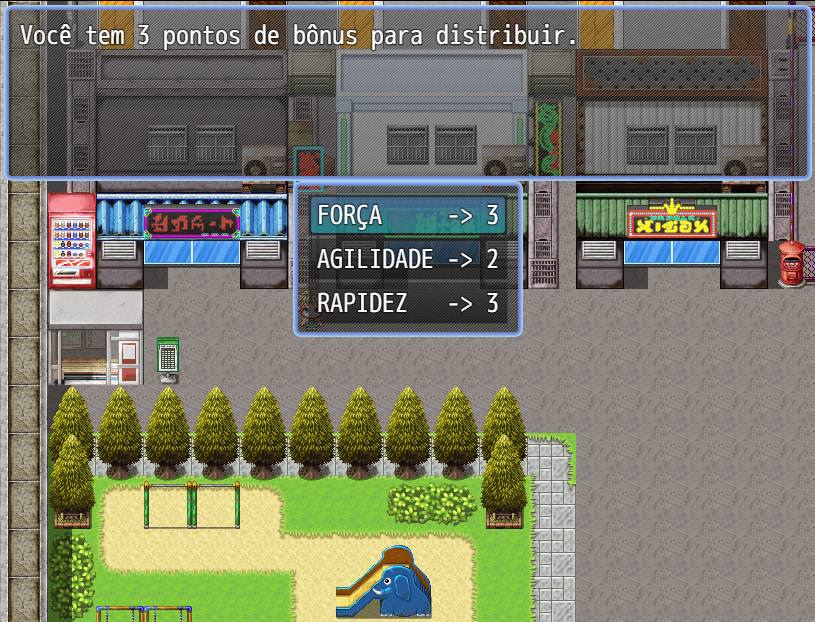
\includegraphics[scale=0.55]{Textuais/Pictures/Distribui-bonus.png}
	\fonte{Elaborado pelo autor (2023).}\label{fig:distribui-bonus}
\end{figure}

Após a distribuição dos pontos de bônus, o jogador é inserido na narrativa, onde necessita tomar decisões cruciais. A primeira decisão é a escolha de um relógio: um modelo funcional e econômico por R\$ 30,00 ou o relógio do Major Trovão, mais caro (R\$ 45,00) e popular entre os colegas. Essa escolha, ilustrada na Figura~\ref{fig:escolha-relogio}, influencia o desenrolar da história, pois a aquisição do relógio mais caro limita os recursos financeiros para a compra de outros itens, como a lanterna necessária para a exploração do porão.

\begin{figure}[!htbp]
	\centering
	\caption{Escolha do relógio.}
	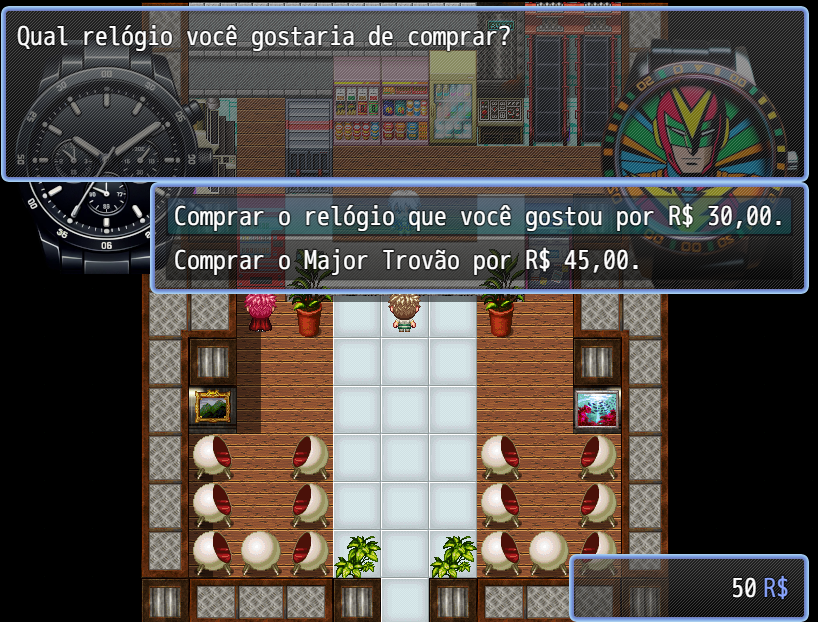
\includegraphics[scale=0.5]{Textuais/Pictures/escolha-relogio.png}
	\fonte{Elaborado pelo autor (2023).}\label{fig:escolha-relogio}
\end{figure}

Posteriormente, o jogador se dirige à lanchonete para um encontro com amigos, ocasião em que gasta R\$ 5,00. Essa etapa é retratada na Figura~\ref{fig:lanchonete-pos-relogio}, e dependendo da escolha do relógio, o jogador pode ter recursos limitados.%, conforme demonstrado na figura~\ref{fig:lanchonete-pos-relogio-mt}.

\begin{figure}[!htbp]
	\centering
	\caption{Lanche pós-escolha do relógio econômico.}
	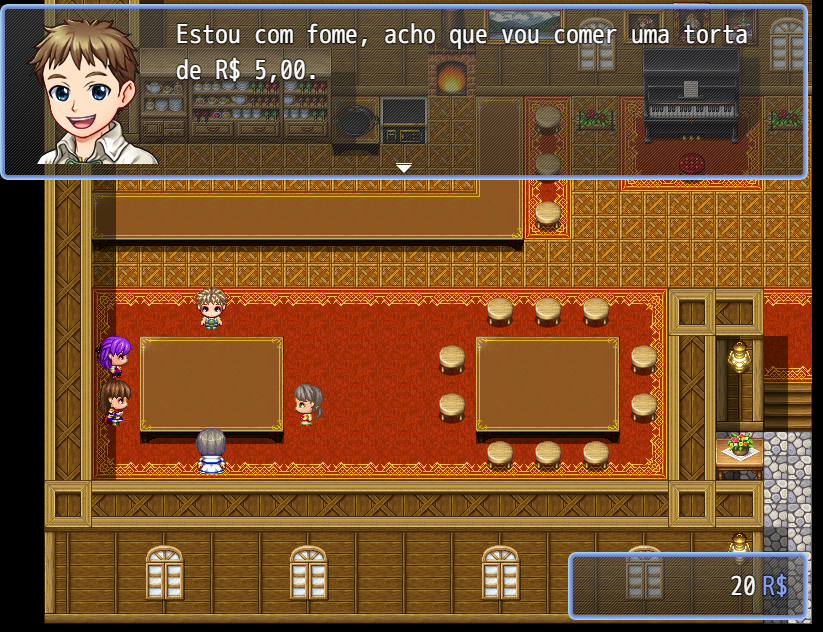
\includegraphics[scale=0.5]{Textuais/Pictures/lanchonete-pos-relogio.png}
	\fonte{Elaborado pelo autor (2023).}\label{fig:lanchonete-pos-relogio}
\end{figure}

A próxima fase do jogo envolve a compra de uma lanterna por R\$ 10,00, essencial para investigar o porão da papelaria. A capacidade do jogador de adquirir a lanterna depende das escolhas financeiras anteriores, como representado nas Figuras~\ref{fig:compra-lanterna} e~\ref{fig:nao-compra-lanterna}.

\begin{figure}[!htbp]
	\centering
	\caption{Aquisição da lanterna.}
	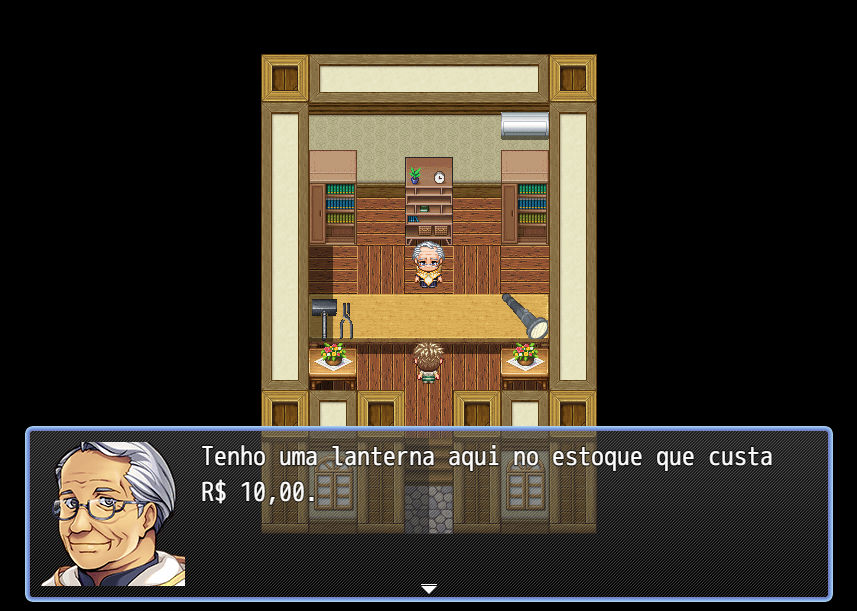
\includegraphics[scale=0.5]{Textuais/Pictures/compra-lanterna.png}
	\fonte{Elaborado pelo autor (2023).}\label{fig:compra-lanterna}
\end{figure}

\begin{figure}[!htbp]
	\centering
	\caption{Incapacidade de comprar a lanterna.}
	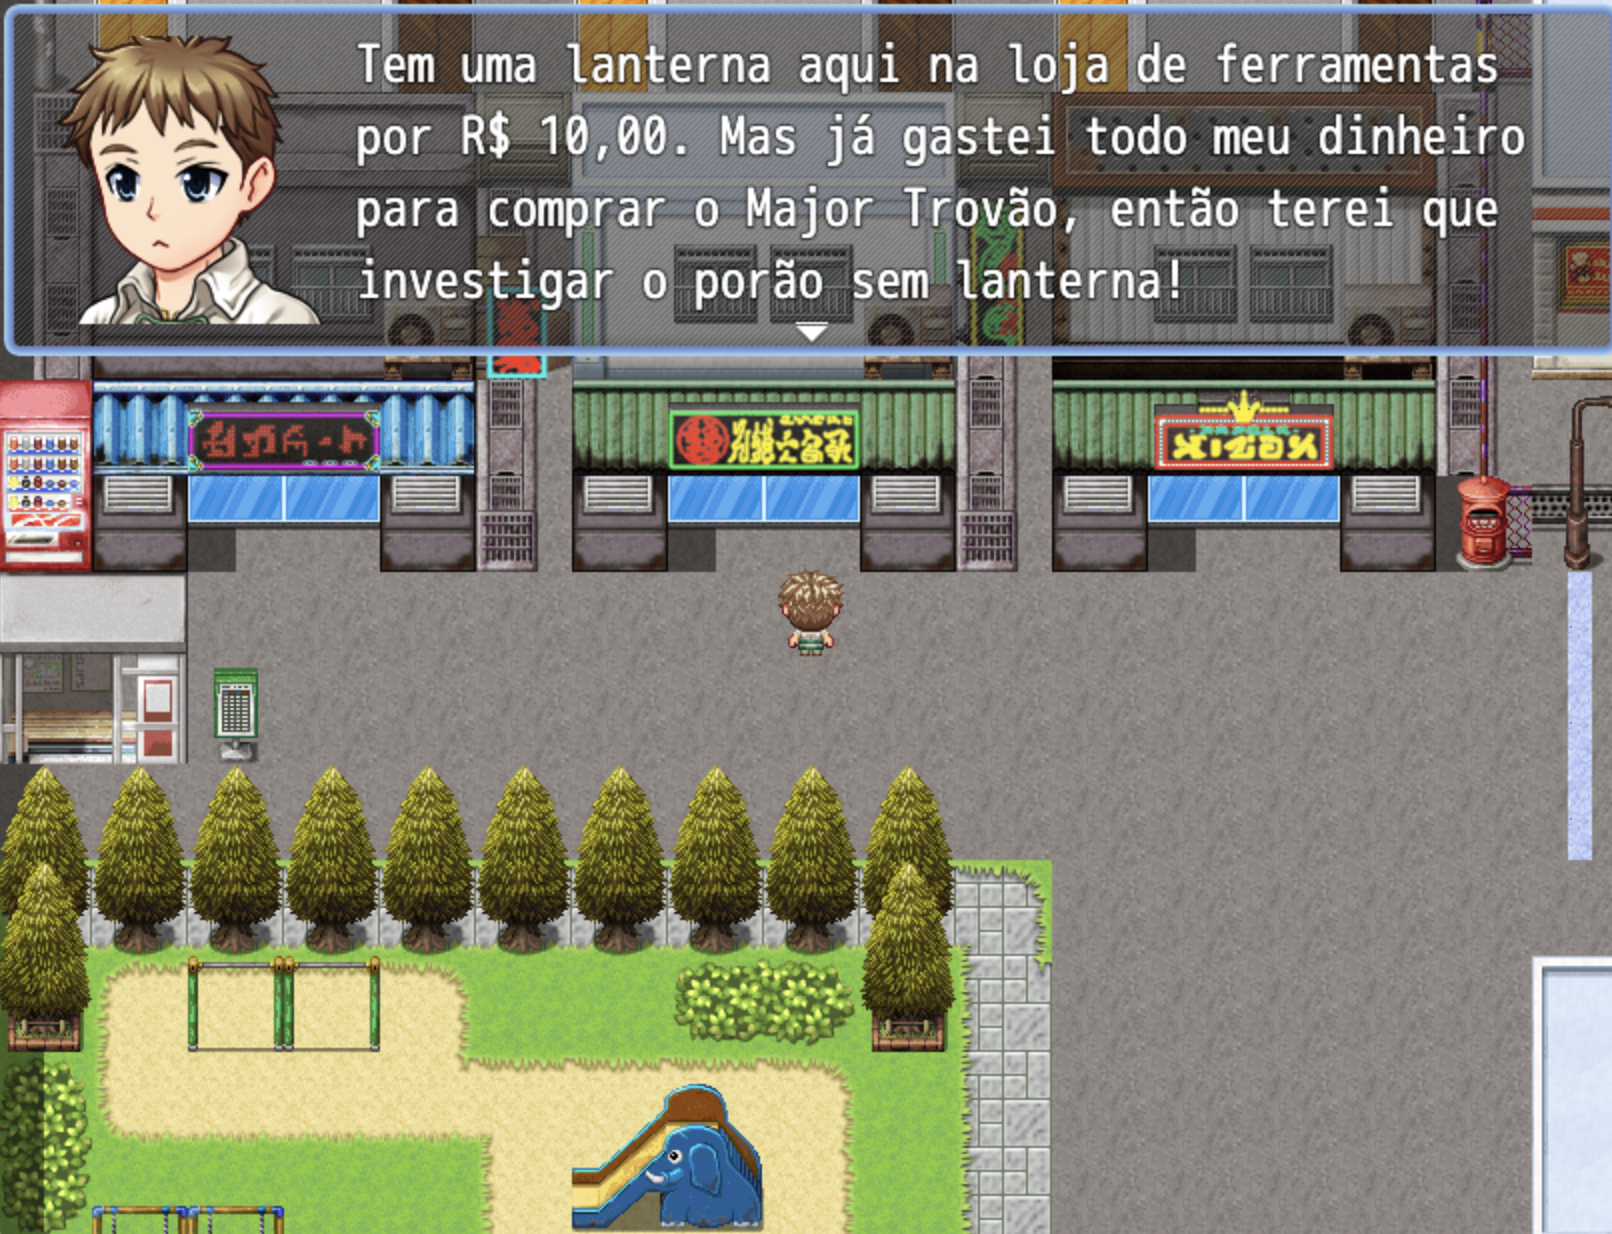
\includegraphics[scale=0.4]{Textuais/Pictures/nao-compra-lanterna.png}
	\fonte{Elaborado pelo autor (2023).}\label{fig:nao-compra-lanterna}
\end{figure}

Após a aquisição (ou não) da lanterna, o personagem principal chega à papelaria e se depara com um barulho na cozinha. Nesse momento, é apresentada uma escolha crítica ao jogador, ilustrada na Figura~\ref{fig:chega-cozinha-papelaria}: investigar a cozinha ou prosseguir diretamente para o porão. Na cozinha, o jogador encontra Josimar e, após sua saída, descobre um problema na geladeira que gera desperdício de energia. Esta descoberta é representada na Figura~\ref{fig:desperdicio-geladeira}.

\begin{figure}[!htbp]
	\centering
	\caption{Decisão entre investigar a cozinha ou ir direto ao porão.}
	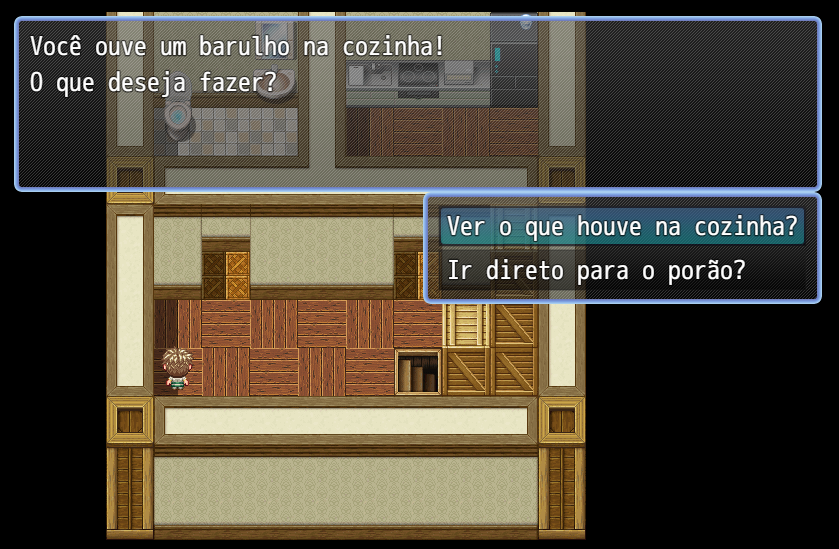
\includegraphics[scale=0.45]{Textuais/Pictures/chega-cozinha-papelaria.png}
	\fonte{Elaborado pelo autor (2023).}\label{fig:chega-cozinha-papelaria}
\end{figure}

\begin{figure}[!htbp]
	\centering
	\caption{Descoberta do desperdício de energia pela geladeira.}
	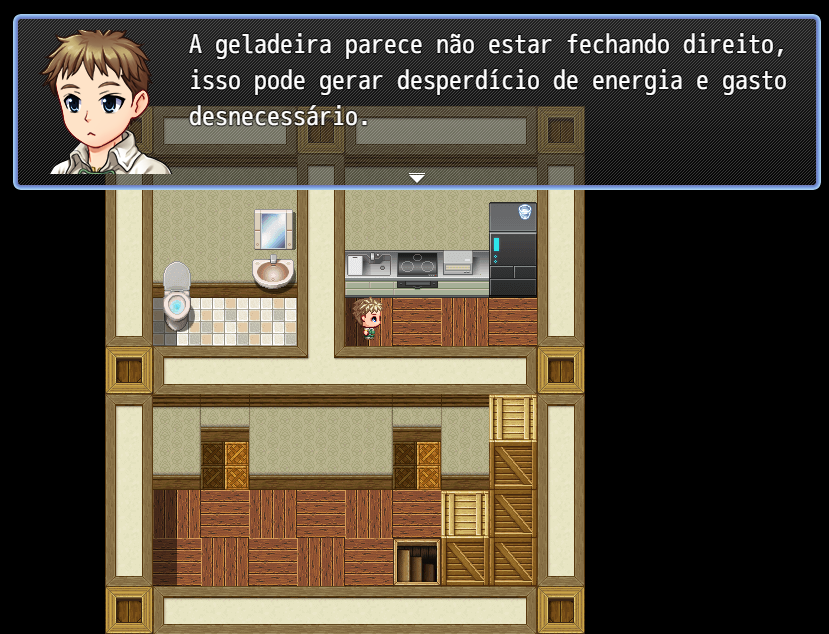
\includegraphics[scale=0.45]{Textuais/Pictures/desperdicio-geladeira.png}
	\fonte{Elaborado pelo autor (2023).}\label{fig:desperdicio-geladeira}
\end{figure}

A exploração do porão pode ocorrer com ou sem a lanterna, conforme as Figuras~\ref{fig:explorando-porao-com-lanterna} e~\ref{fig:explorando-porao-sem-lanterna}. A falta de lanterna e uma baixa pontuação em agilidade podem levar a um ataque de ratazana, culminando em um final prematuro do jogo, como mostrado na Figura~\ref{fig:game-over}.

\begin{figure}[!htbp]
	\centering
	\caption{Exploração do porão com a lanterna.}
	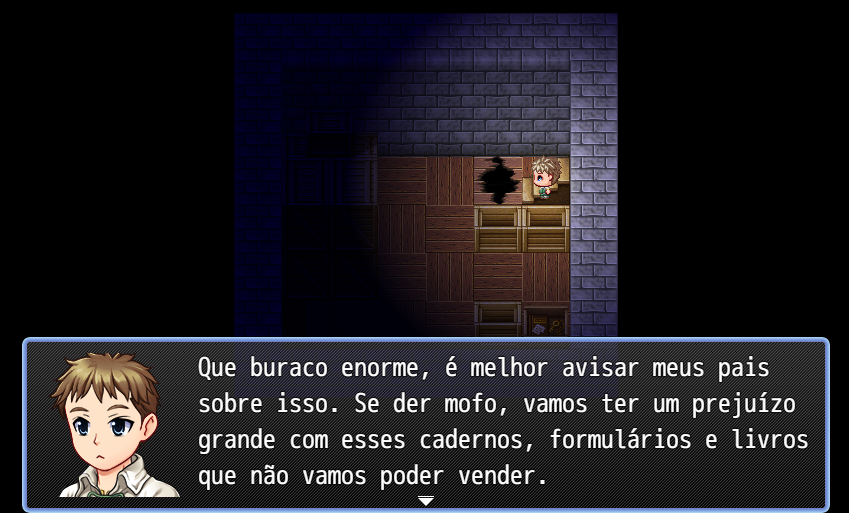
\includegraphics[scale=0.55]{Textuais/Pictures/explorando-porao-com-lanterna.png}
	\fonte{Elaborado pelo autor (2023).}\label{fig:explorando-porao-com-lanterna}
\end{figure}

\begin{figure}[!htbp]
	\centering
	\caption{Exploração do porão sem a lanterna.}
	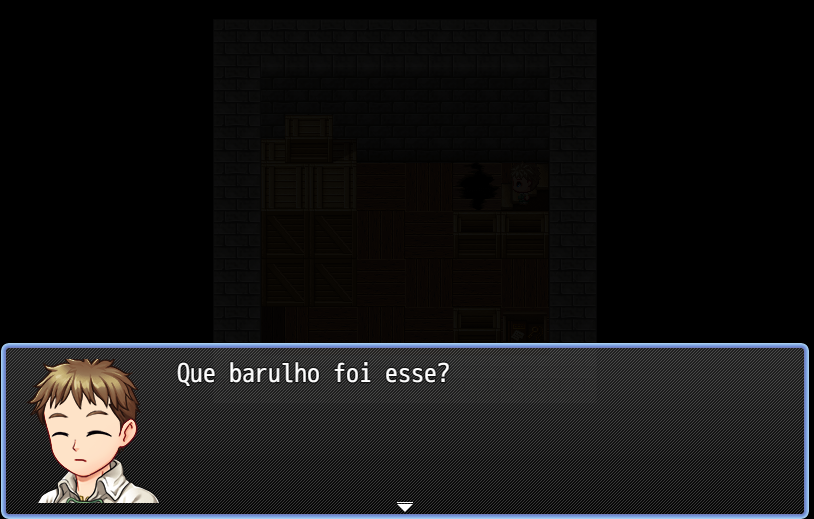
\includegraphics[scale=0.55]{Textuais/Pictures/explorando-porao-sem-lanterna.png}
	\fonte{Elaborado pelo autor (2023).}\label{fig:explorando-porao-sem-lanterna}
\end{figure}

\begin{figure}[!htbp]
	\centering
	\caption{Consequências de uma baixa pontuação em agilidade.}
	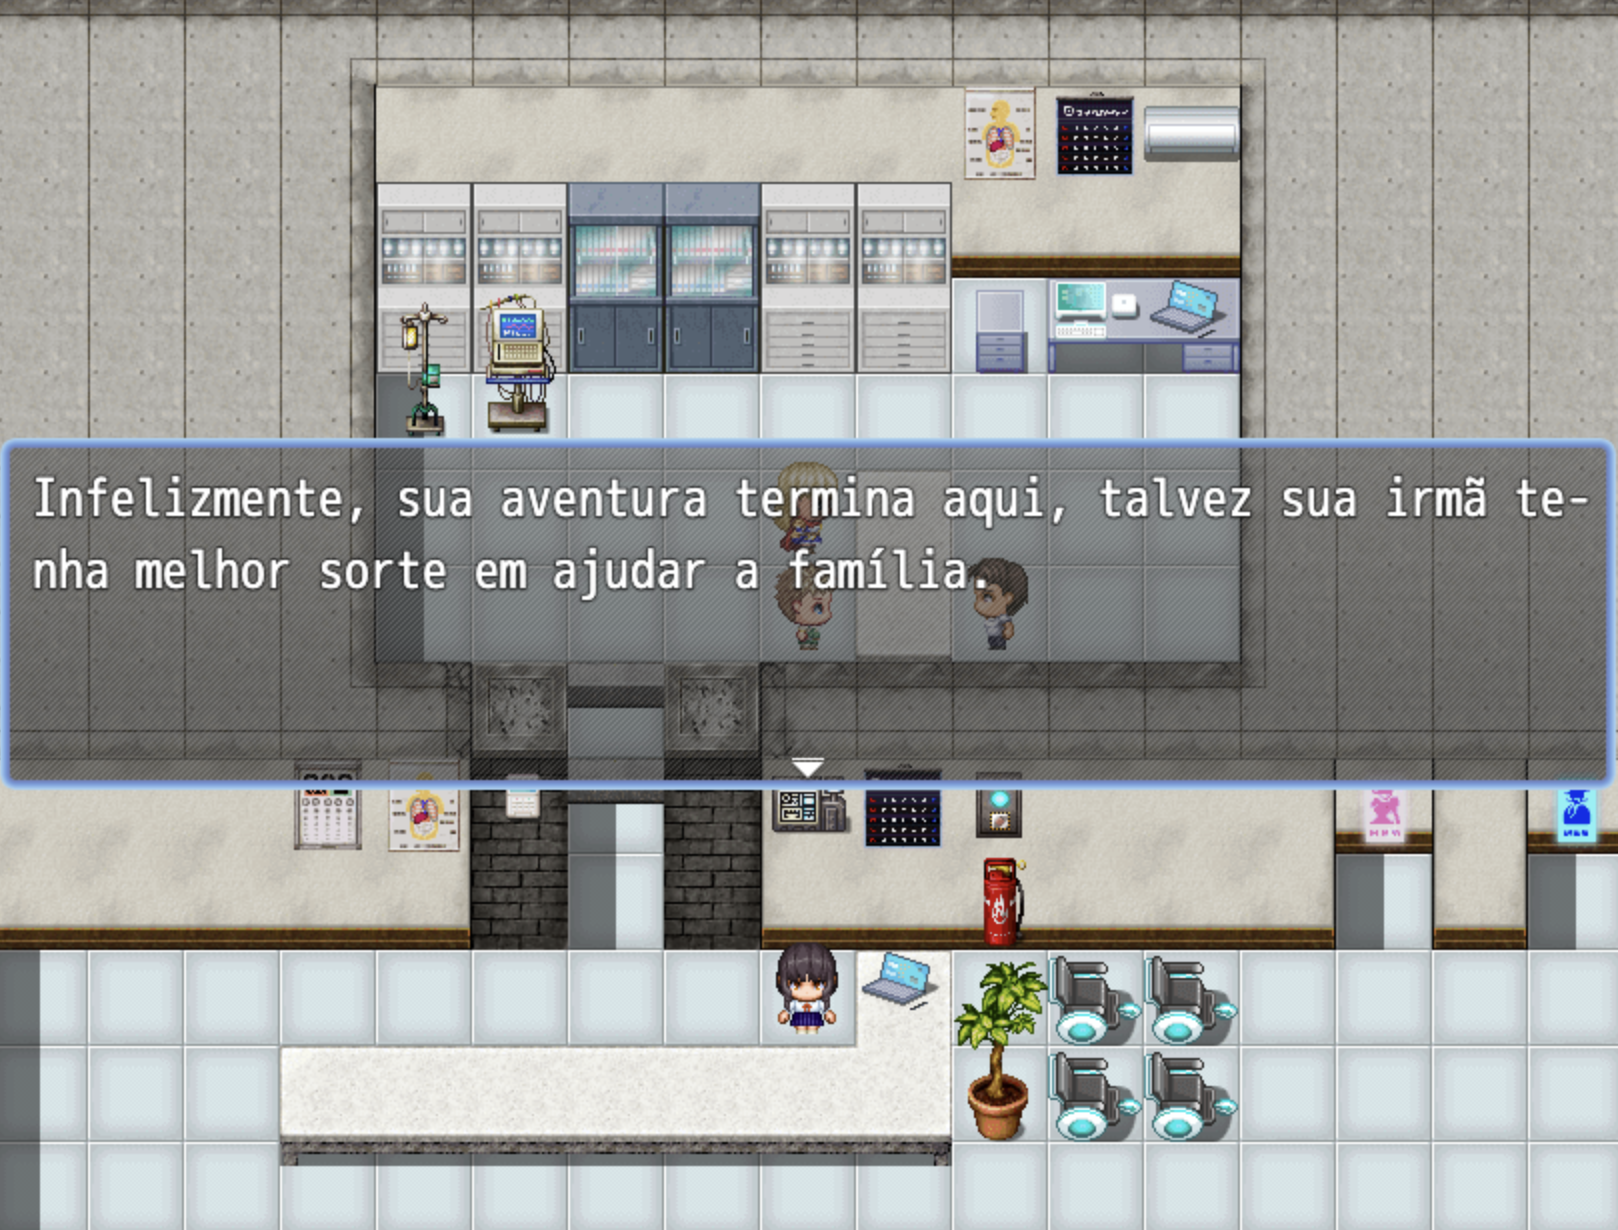
\includegraphics[scale=0.4]{Textuais/Pictures/game-over.png}
	\fonte{Elaborado pelo autor (2023).}\label{fig:game-over}
\end{figure}

Se o jogador realizar escolhas adequadas ao longo do jogo, alcança um desfecho positivo. A família descobre a origem dos problemas financeiros e encontra as moedas esquecidas, solucionando o mistério. Esse desfecho vitorioso é ilustrado na Figura~\ref{fig:vitoria}.

\begin{figure}[!htbp]
	\centering
	\caption{Conclusão bem-sucedida do jogo.}
	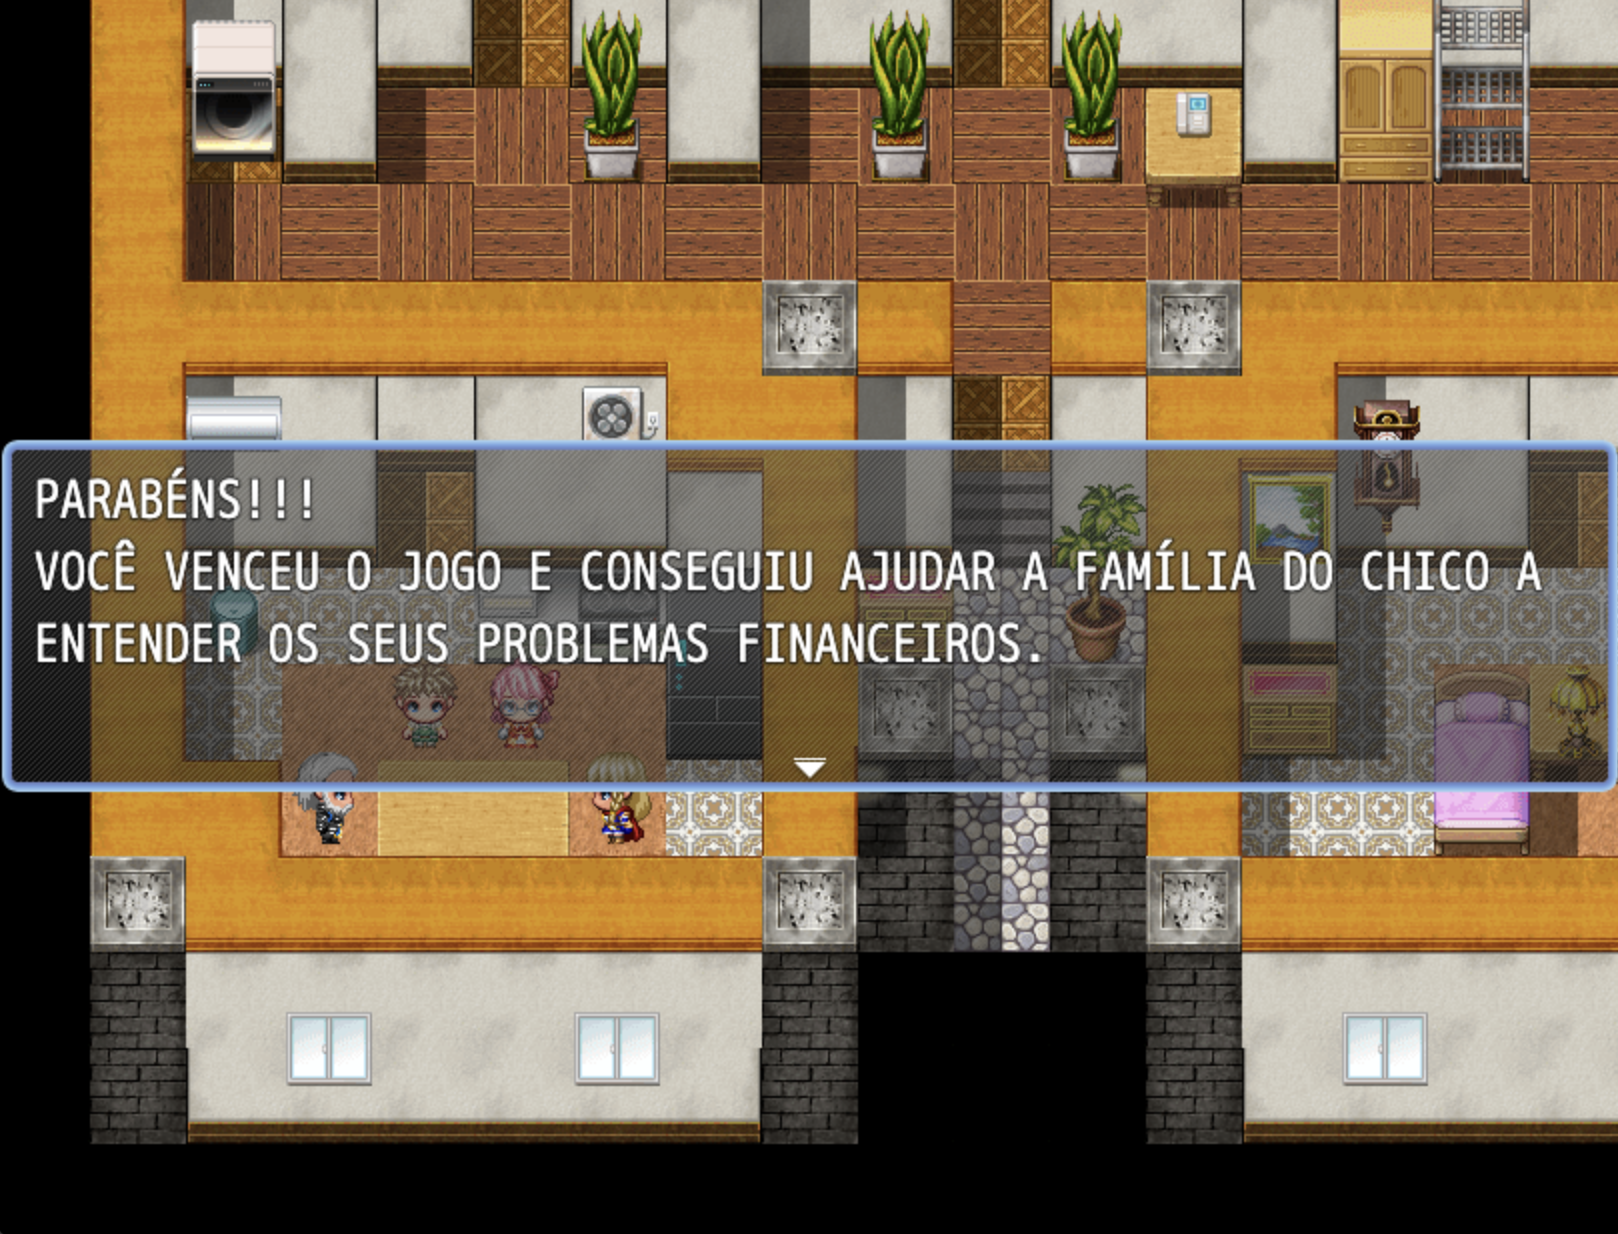
\includegraphics[scale=0.4]{Textuais/Pictures/vitoria.png}
	\fonte{Elaborado pelo autor (2023).}\label{fig:vitoria}
\end{figure}

\section{Análise Crítica}

Esta seção apresenta uma análise do jogo desenvolvido, comparando com os trabalhos correlatos. Os jogos são analisados segundo diferentes aspectos, como público-alvo, abordagem pedagógica e imersão do jogador.

Quanto ao \textbf{público-alvo}, o jogo \textit{Mistério Financeiro} é direcionado para crianças do 5º ano do Ensino Fundamental, demandando abordagens educativas lúdicas e interativas. Esse foco no público infantil o diferencia de jogos como \textit{Debt Maze} (Seção~\ref{subsec:debt-maze}) e \textit{Finance Game} (Seção~\ref{subsec:finance-game}), mais apropriados para adultos ou adolescentes.

Quanto à \textbf{metodologia de ensino}, ao contrário do \textit{PlanCash} (Seção~\ref{subsec:plancash}), que utiliza uma estrutura de jogo de tabuleiro, e do \textit{InvestPlay} (Seção~\ref{subsec:investplay}), baseado em perguntas e respostas, o jogo \textit{Mistério Financeiro} emprega uma narrativa interativa no formato de RPG. Essa abordagem é particularmente eficaz para engajar crianças mais jovens~\cite{liu2017intelligent}.

Em relação à \textbf{abordagem pedagógica}, o jogo promove aprendizagem por meio da exploração e tomada de decisões, similar ao \textit{Debt Maze}, mas de uma forma mais acessível e relevante para o público infantil. As situações financeiras são integradas naturalmente na narrativa, facilitando a compreensão e retenção de conhecimento.

Em relação à \textbf{imersão}, a rica narrativa de Chico e sua família em \textit{Mistério Financeiro} oferece uma experiência imersiva, em contraste com o \textit{PlanCash}, cujo formato de jogo de tabuleiro pode limitar o envolvimento narrativo e, por consequência, o engajamento e o aprendizado.

No que diz respeito à \textbf{contextualização cultural e linguística}, o jogo \textit{Mistério Financeiro} se destaca pela sua forte contextualização no cenário brasileiro e uso do português como idioma principal, diferenciando-se de jogos como o \textit{Debt Maze}, que apresentam barreiras linguísticas para o público brasileiro.

Quanto à \textbf{aderência à ENEF}, este é um ponto forte do jogo \textit{Mistério Financeiro}. Ele está alinhado com os princípios da Estratégia Nacional de Educação Financeira (ENEF), ao contrário dos outros jogos analisados. Esta conformidade assegura que o conteúdo e as lições financeiras estejam em harmonia com os objetivos educacionais nacionais.

Apesar de suas vantagens, é importante destacar alguns \textbf{pontos fracos} do jogo \textit{Mistério Financeiro}. O jogo ainda carece de avaliação empírica com estudantes, o que limita a validação da sua eficácia educacional. Além disso, a narrativa específica pode restringir a re-jogabilidade e a variedade dos cenários financeiros explorados.

Em resumo, a análise comparativa apresentada revela que o jogo \textit{Mistério Financeiro} oferece uma abordagem inovadora e adequada para o seu público-alvo, distinguindo-se significativamente dos outros jogos analisados em termos de metodologia, abordagem pedagógica, imersão narrativa, contextualização cultural e aderência à ENEF. Cada jogo tem seus pontos positivos, mas o \textit{Mistério Financeiro} se sobressai pela sua integração única de educação financeira com uma narrativa envolvente, ajustada ao contexto cultural brasileiro.